\documentclass[a4paper, 12pt]{article}

\usepackage{graphicx}
\usepackage[font=small, labelfont=bf, labelsep=colon]{caption}
\usepackage{amsmath, amssymb}
\usepackage{float}
\usepackage{textcomp}
\usepackage{siunitx}
\usepackage[dvipsnames]{xcolor}
\usepackage{titling} % To allow to use \matitle more than once
\usepackage{ctable}
\usepackage{multirow}
\usepackage[flushmargin, bottom]{footmisc} 
\usepackage{hyperref}
\usepackage{cleveref}


\hypersetup{
colorlinks = true,
linkcolor = {blue!80!black}
}

\graphicspath{{../../../Pictures/}}

%%%%%%%%%%%%%%%%%%%%%%%%%%%%%%%%%%%%%%%%%%%%%%%%%%%%%%%
% Layout parameters 
\setlength{\parindent}{0em}
\setlength{\parskip}{2ex}
\linespread{1.2}

\renewcommand{\floatpagefraction}{.99} % Minimum fraction of floats, in a page that has only floats. Only figures taking up more than that will get their own page. Default 0.5
\renewcommand{\topfraction}{0.99}  % Maximum fraction of page for floats at top. I.e.: floats taking up more than this will have no text below. Default: 0.7.
\renewcommand{\textfraction}{0.01} % Minimum fraction of page that must have text (otherwise, the page will only have float). Default: 0.2 

\addtolength{\textwidth}{2cm}
\addtolength{\hoffset}{-1cm}
\setlength{\topmargin}{-1cm}
\addtolength{\textheight}{1cm}

\setlength{\skip\footins}{6mm} % space between end of text and horizontal line of footnote
\setlength{\footnotesep}{5mm} % space between footnote line and first entry, and between consecutive entries of footnote



%%%%%%%%%%%%%%%%%%%%%%%%%%%%%%%%%%%%%%%%%%%%%%%%%%

%%%%%%%%%%%%%%%%%%%%%%%%
%%%%% NEW COMMANDS
%%%%%%%%%%%%%%%%%%%%%%%%

% Text commands
\newcommand{\spc}{1ex}
\newcommand{\eg}{\textit{e.g.}}
\newcommand{\ie}{\textit{i.e.}}

% Maths Commands
\newcommand{\R}{\mathbb{R}}
\newcommand{\bd}[1]{\boldsymbol{#1}}
\newcommand{\x}{\bd x}
\newcommand{\A}{{_{[A]}}}
\newcommand{\xA}{\bd{x^\A}}
\newcommand{\eps}{\varepsilon}
\newcommand{\Nr}{N_\text{regr}}
\newcommand{\E}{\mathbb{E}}
\newcommand{\Var}{\text{Var}}

\newcommand{\D}{\mathcal{D}}


\newcommand{\ya}{y^{(\alpha)}}
\newcommand{\yb}{y^{(\beta)}}
\newcommand{\ta}{\bd{\widetilde \alpha}}
\newcommand{\tb}{\bd{\widetilde \beta}}



%%%%%%%%%%%%%%%%%%%%%%%%%%%%%%%%%%%%%%%%%%%%%%%%%%%%%

\title{New Emulators for Monthly Gas Consumption}

\author{}
\date{}

\begin{document}

\maketitle
\vspace{-9ex}


This document is a concise summary of the construction and validation of the monthly gas consumption emulators. 
The 1000 design runs are divided into three sets:
\begin{itemize}
\item Training set (700 runs): used to train the emulators which predict the simulator's response on any other run;
\item Evaluation set (150 runs): used to choose the values of the emulator hyperparameters, by comparing the emulator's performance on the set with the know simulator's outputs;
\item Test set (150 runs): used to test the previously built emulators on a completely new set of runs not used in training and evaluation.
\end{itemize}
\autoref{Table_Var_names} lists the meaning and range of the 8 inputs which are varied from one simulation to the other.

\begin{table}
 \centering
 \renewcommand{\arraystretch}{1.4}
 \newcommand{\colsep}{4ex}
 \caption{Meaning and range of the eight parameters varied among the $n$ simulations of this work. {\it \footnotesize(Mohammad may provide more appropriate descriptions for the middle column.)}}
 \begin{tabular}{c<{\hspace{\colsep}}  c<{\hspace{\colsep}}  c}
\specialrule{.1em}{0em}{0.1em} 
 \textbf{Short Name} &  \textbf{Physical Meaning} & \textbf{Range} \\
 \specialrule{.05em}{.1em}{0.1em} 
 \specialrule{.05em}{0em}{0.2em} 
  $V_1$   &  Heating Setpoint               &  $[17.5, 20.5]$ $\si{\celsius}$        \\
  $V_2$   &  Boiler Efficiency              &  $[0.6, 0.75]$                         \\
  $V_3$   &  External wall thickness        &  $[4, 6.3]$ cm                         \\
  $V_4$   &  Roof quilt thickness           &  $[15, 21]$ cm                         \\
  $V_5$   &  Floor insulation thickness     &  $[4.5, 5.5]$ cm                       \\
  $V_6$   &  Infiltration rate              &  $[0.2, 0.95]$ ac/h                    \\
  $V_7$   &  DHW Consumption                &  $[6.15, 22] \!\times\! 10^{-6}$ litre/day \\
  $V_8$   &  Cooking                        &  $[1.05, 6.3]$ W/m$^2$                 \\
 \specialrule{.1em}{0.2em}{1em} 
 \end{tabular}
\label{Table_Var_names}
\end{table}

\section{Emulators' Training}
In order to emulate the monthly gas consumption, the range of each of the eight input variables $V_1, \dots, V_8$ has been linearly rescaled into $[-1,1]$.
Given the outputs $y_i$ of the 700 training runs for a given month, 
I have first built a linear regression model of $y_i$ as a function of (some of the) linear, quadratic and interaction terms of the $V_i$.
Hence, I have built an emulator of the linear regression residuals. Details of the two steps follow.

\subsubsection*{Linear Regression}
Let $\mathcal{R}$ be the set of all linear, quadratic and interaction terms of the 8 inputs $V_1, \dots, V_8$, all mutually orthogonal.
As it turns out, for all months, the set of the ``best'' 10 regressors in $\mathcal{R}$ (the set maximising the adjusted $R^2$) explains the data extremely well, 
with an adj-$R^2$ of about 0.999 in all cases. Given the excellent result, and to use an approach which is uniform among months and simple to explain,  
for each month I have built a linear regression model by selecting the best 10 regressors according to the above criterion. 
\emph{(previously, for May, I was using some 3rd-order terms to improve the linear model. Probably not worth it)}

\autoref{Table_Regressors} shows which 10 regressors have been selected for each month, the adjusted $R^2$ of the associated linear model, and the variance of the residuals.

\begin{table}
 \centering
 \renewcommand{\arraystretch}{1.4}
 \newcommand{\colsep}{3ex}
 \caption{For each of the nine months considered, from left to right: the set of covariates used to build the linear regression model, the adjusted $R^2$ of the model, the variance of the residuals.
 In the second column, the ``$\ast$'' symbol is used as shorthand notation to denote all linear and interaction terms, \eg\ $\,a \ast b \ast c = \{ a, b, c , ab, ac, bc \}$.}
 \begin{tabular}{c<{\hspace{\colsep}}  c<{\hspace{\colsep}}  c<{\hspace{\colsep}} c}
\specialrule{.1em}{0em}{0.1em} 
 \textbf{Month} &  \textbf{Regressors} & \textbf{Adj.~$R^2$} & \textbf{Resid.~Var.~$\sigma^2$}\\
 \specialrule{.05em}{.1em}{0.1em} 
 \specialrule{.05em}{0em}{0.2em} 
  Jan  &  $V_1 \!\ast\! V_2 \!\ast\! V_6, \,V_3,\, V_4,\,{V_2}^2,\, {V_6}^2$   & 0.9998   & 85.94\\
  Feb  &  $V_1 \!\ast\! V_2 \!\ast\! V_6, \,V_3,\, V_4,\,{V_2}^2,\, {V_6}^2$   & 0.9998  &  52.30\\
  Mar  &  $V_1 \!\ast\! V_2 \!\ast\! V_6, \,V_3,\, V_4,\,{V_2}^2,\, {V_6}^2$   & 0.9997  &  50.14\\
  Apr  &  $V_1 \!\ast\! V_2 \!\ast\! V_6, \,V_3,\, V_4,\,{V_2}^2,\, {V_6}^2$   & 0.9998  &  50.04\\  
  May  &  $V_1 \!\ast\! V_2 \!\ast\! V_6, \,V_3,\, V_8,\,{V_1}^2,\, {V_6}^2$   & 0.9989  & 206.45\\
  Sep  &  $V_1 \!\ast\! V_2 \!\ast\! V_6, \,V_3,\, V_4,\, V_8,\, {V_6}^2$         & 0.9994  &  0.91\\
  Oct  &  $V_1 \!\ast\! V_2 \!\ast\! V_6, \,V_3,\, V_4,\, V_8,\, {V_6}^2$         & 0.9996  &  24.40\\
  Nov  &  $V_1 \!\ast\! V_2 \!\ast\! V_6, \,V_3,\, V_4,\,{V_2}^2,\, {V_6}^2$   & 0.9998 &  57.35\\
  Dec  &  $V_1 \!\ast\! V_2 \!\ast\! V_6, \,V_3,\, V_4,\,{V_2}^2,\, {V_6}^2$   & 0.9998  &  68.77\\
 \specialrule{.1em}{0.2em}{1em} 
 \end{tabular}
\label{Table_Regressors}
\end{table}


\subsubsection*{Bayes Linear Emulators of Residuals}
In order to build an emulator of the residuals, choices about the following are to be made: active inputs, correlation lengths, prior emulator variance and nugget variance.

To choose these, for each month, I have followed the general procedure which I highlight below. In particular, the procedure to choose active inputs and correlation lengths has involved visual assessment of the emulator's performance on the evaluation set, by plotting the standardised residuals for the runs of this set. \autoref{Validation} will provide details and graphs on this. 

\begin{itemize}
\item {\bf Active Inputs}: To identify which inputs were significant in explaining the residuals, I have looked at the best selection of second- (and sometimes third-) order terms in a linear regression model. 
Terms which would appear alone with a significant $t$-value ($t>8$) would be included as an active input; the inclusion of terms appearing only in interaction with other terms or with a low $t$-value would instead be considered case by case, according to the emulator performance on the evaluation set.
\item {\bf Correlation lengths}: Once the active inputs have been chosen, I have used the same correlation length for all of them. The correlation length has been chosen by assessing the emulator's performance on the validation set, also accounting for the number of active inputs used
(to attain a similar level of correlation across the space, higher correlation lengths are needed if more active inputs are used).
\item {\bf Prior Variances}: The cumulative prior variance (the one of the second-order stochastic process over which we make specifications, plus the one of the ``nugget'' process) has been imposed to be the variance of the residuals which are being fitted. This overall variance has been split into the two components in the proportions of $95\%$ and $5\%$, respectively.
\end{itemize}

\autoref{Table_Emulator_Specifications} shows the choices of the above quantities for the nine months of interest.
\autoref{Fig_Correlation} instead gives an idea of the level of correlation across the input space induced by the above choices. Specifically, named $P$ the point at the centre of the hypercube with edges $[-1,1]$, the figure shows histograms of the correlation between the point $P$ and 2 million uniformly distributed points in the hypercube.



\begin{table}
 \centering
 \renewcommand{\arraystretch}{1.4}
 \newcommand{\colsep}{3ex}
 \caption{For each of the nine months considered, the table below shows which active inputs have been chosen and the value of the correlation length (same for all active inputs).}
 \begin{tabular}{c<{\hspace{\colsep}}  c<{\hspace{\colsep}}  c<{\hspace{\colsep}} c}
\specialrule{.1em}{0em}{0.1em} 
 \textbf{Month} &  \textbf{Active Inputs} & \textbf{Corr.~Length}\\
 \specialrule{.05em}{.1em}{0.1em} 
 \specialrule{.05em}{0em}{0.2em} 
  Jan  &  $V_1, \,V_2, \,V_3, \,V_6, \,V_8$               &  0.8\\
  Feb  &  $V_1, \,V_2, \,V_3, \,V_7, \,V_8$               &  0.65\\
  Mar  &  $V_1, \,V_2, \,V_3, \,V_6, \,V_7, \,V_8$   &  1.3\\
  Apr  &  $V_1, \,V_2, \,V_3, \,V_6, \,V_8$              &  1.0\\  
  May  &  $V_1, \,V_2, \,V_3, \,V_4, \,V_6, \,V_8$  &  1.0\\
  Sep  &  $V_1, \,V_2, \,V_3, \,V_6, \,V_7, \,V_8$   &  1.2\\
  Oct  &  $V_1, \,V_2, \,V_3, \,V_6, \,V_7, \,V_8$   &  1.4\\
  Nov  & $V_1, \,V_2, \,V_3, \,V_6, \,V_7, \,V_8$   & 1.2\\
  Dec  &  $V_1, \,V_2, \,V_3, \,V_6, \,V_7, \,V_8$  & 1.3\\
 \specialrule{.1em}{0.2em}{1em} 
 \end{tabular}
\label{Table_Emulator_Specifications}
\end{table}


\newcommand{\scale}{12.7em}
\begin{figure}
\centering
 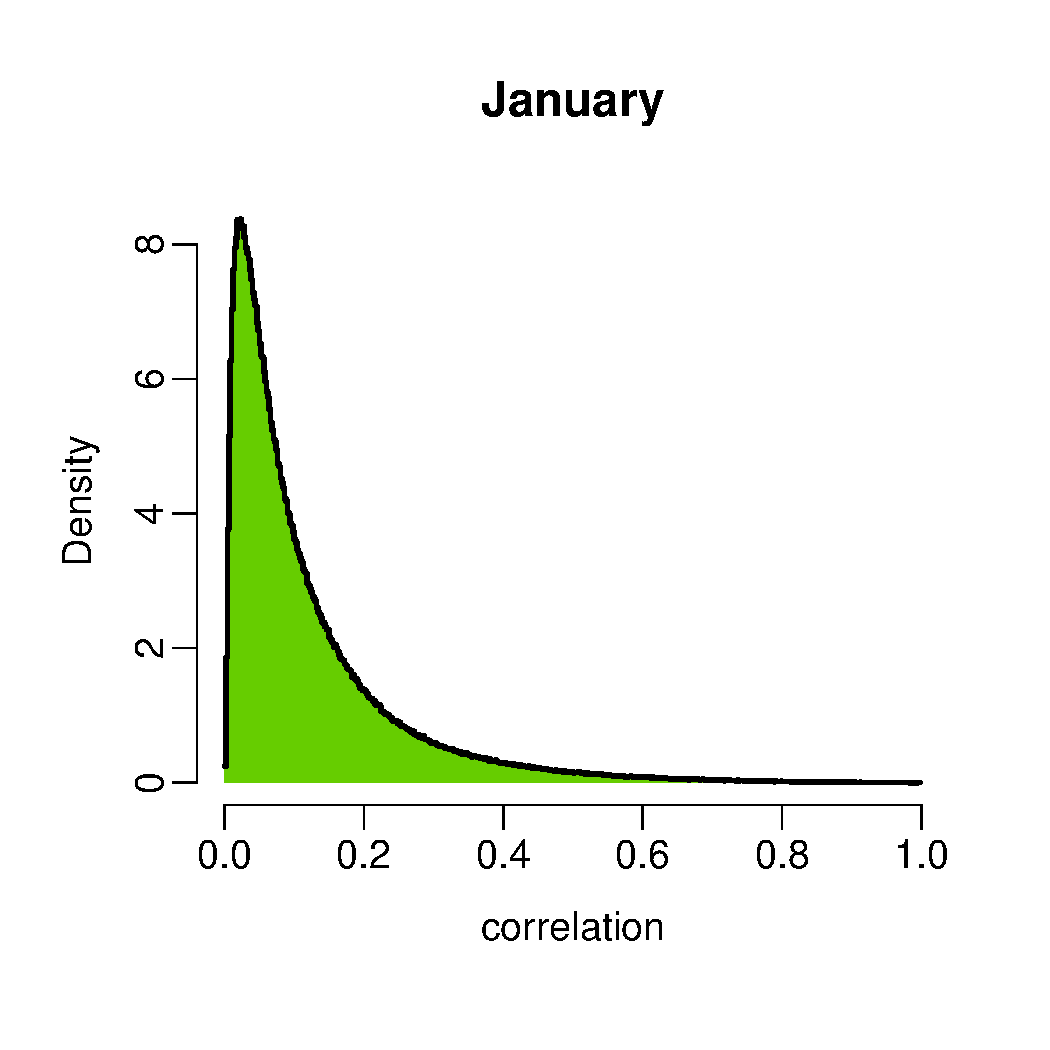
\includegraphics[width=\scale]{Validation_Plots/Correlation/Correlation_01_Jan}\hspace{-1ex}
 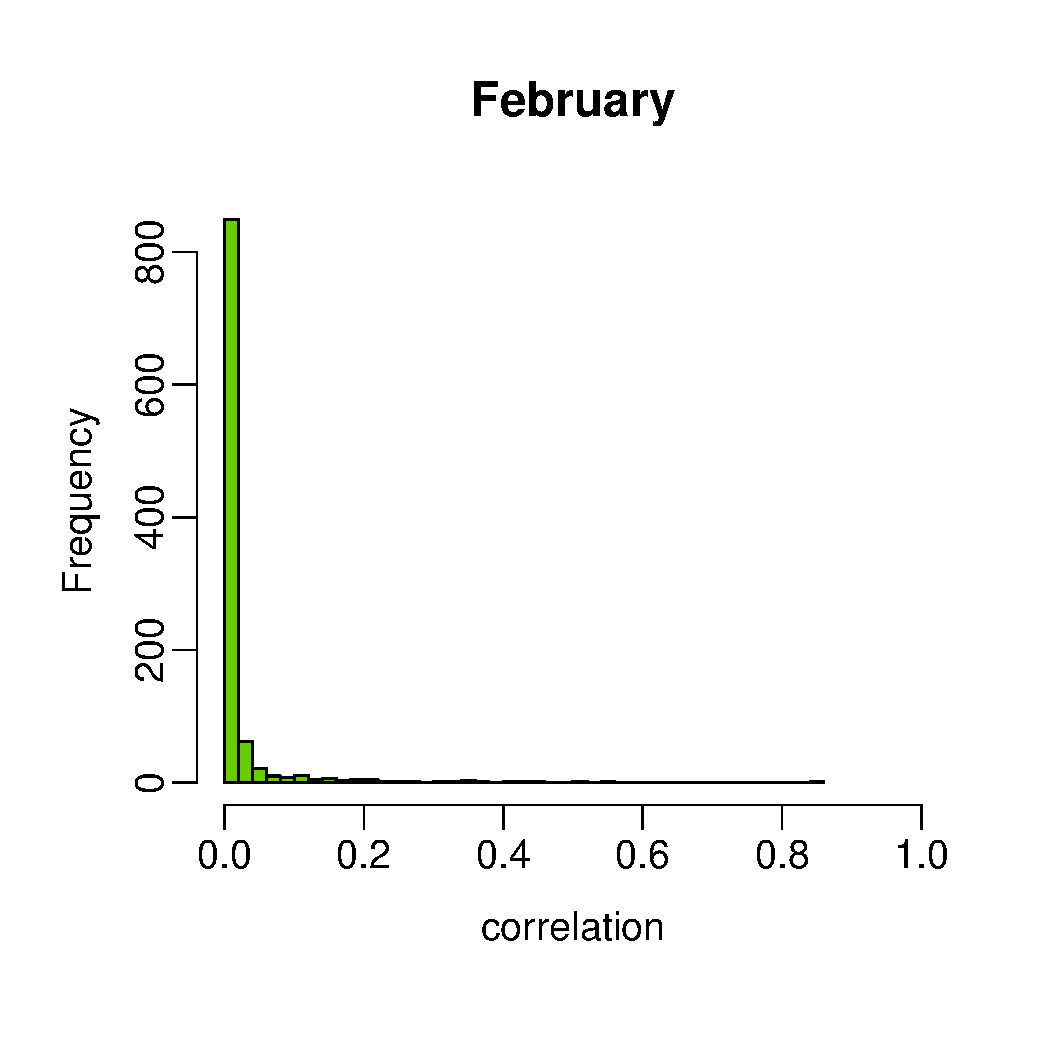
\includegraphics[width=\scale]{Validation_Plots/Correlation/Correlation_02_Feb}\hspace{-1ex}
 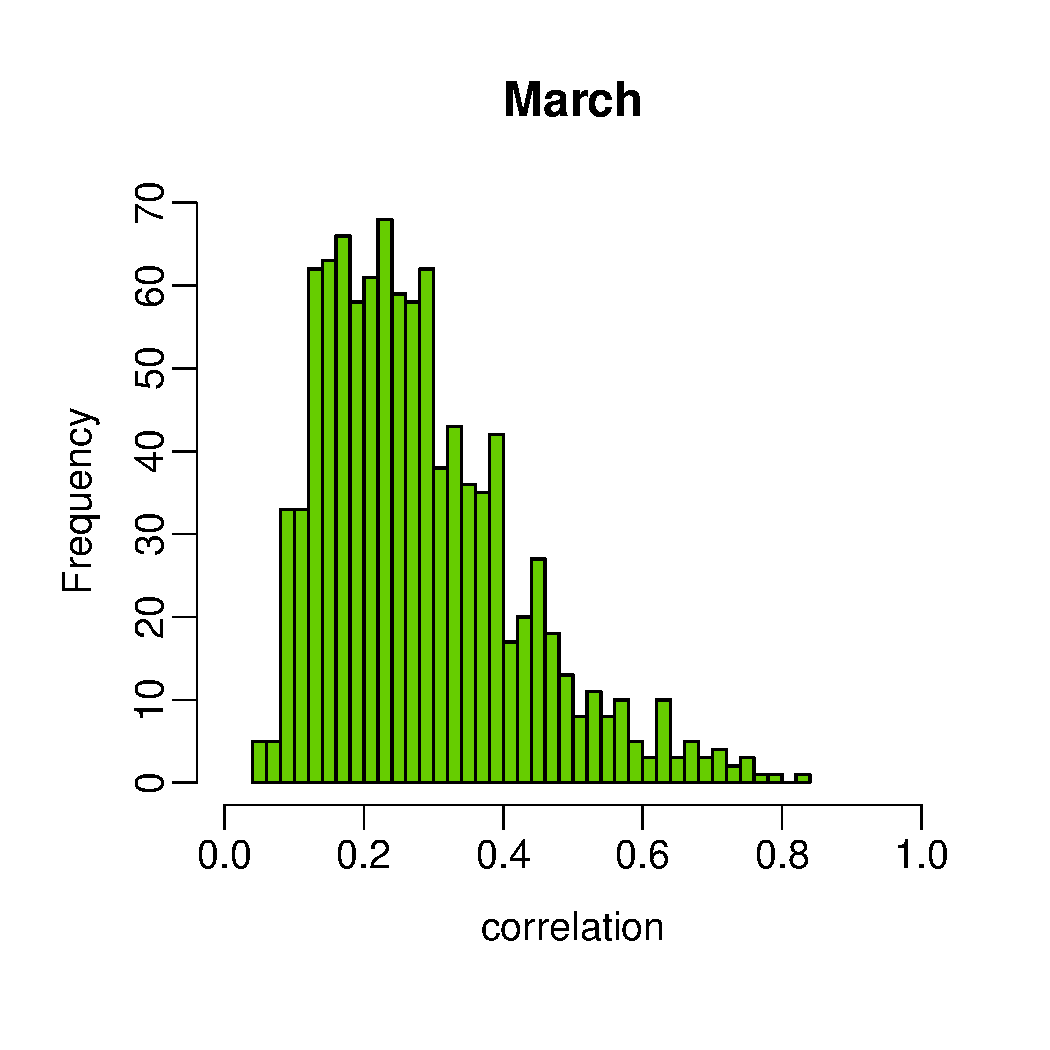
\includegraphics[width=\scale]{Validation_Plots/Correlation/Correlation_03_Mar}\\[-3ex]
 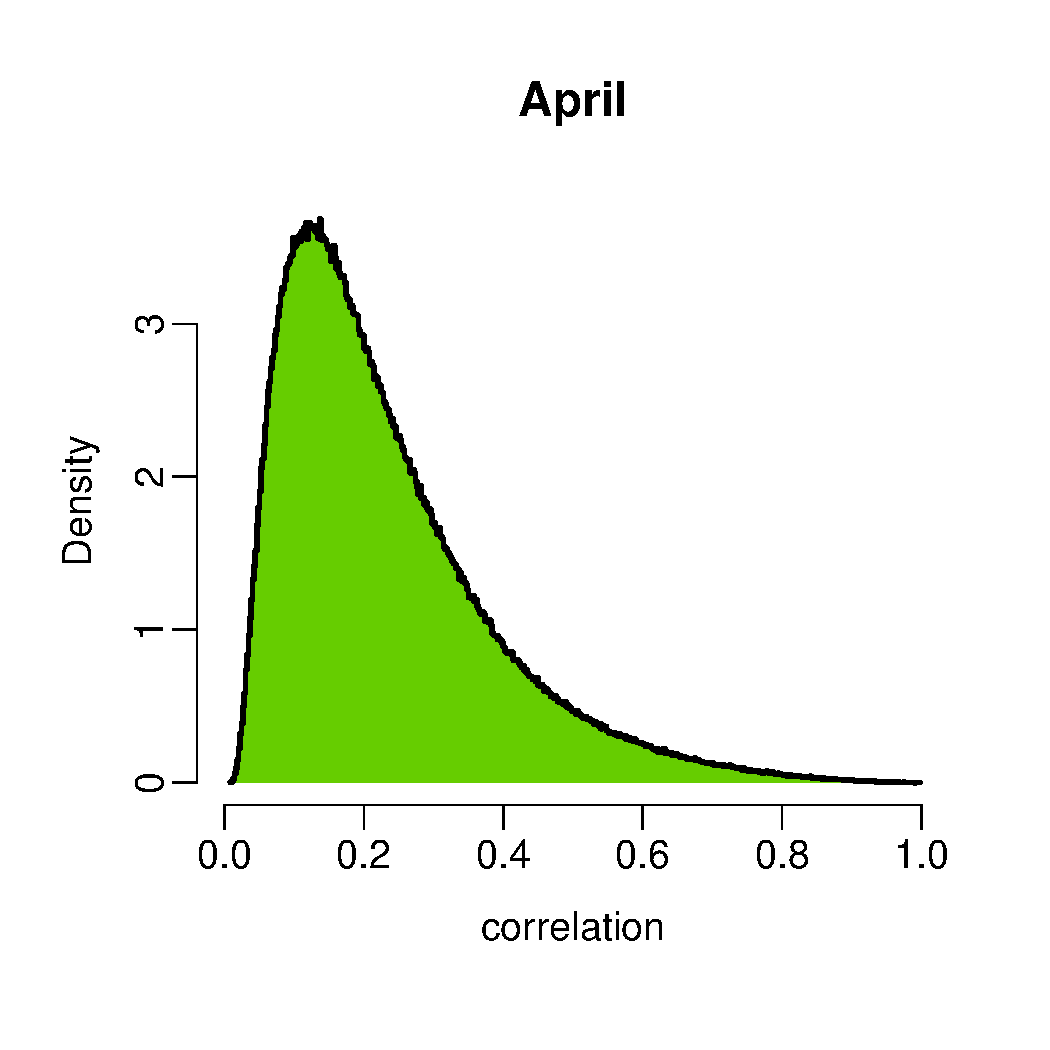
\includegraphics[width=\scale]{Validation_Plots/Correlation/Correlation_04_Apr}\hspace{-1ex}
 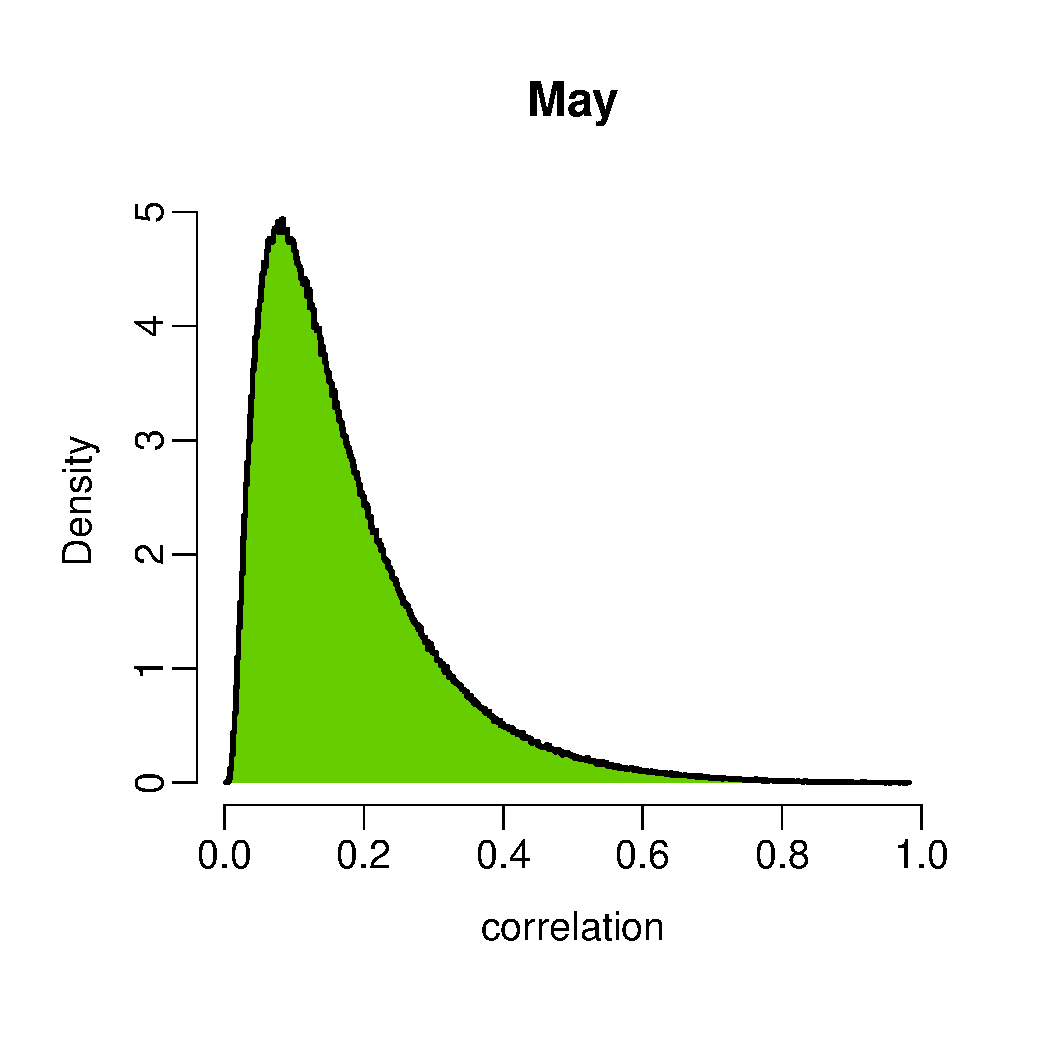
\includegraphics[width=\scale]{Validation_Plots/Correlation/Correlation_05_May}\hspace{-1ex}
 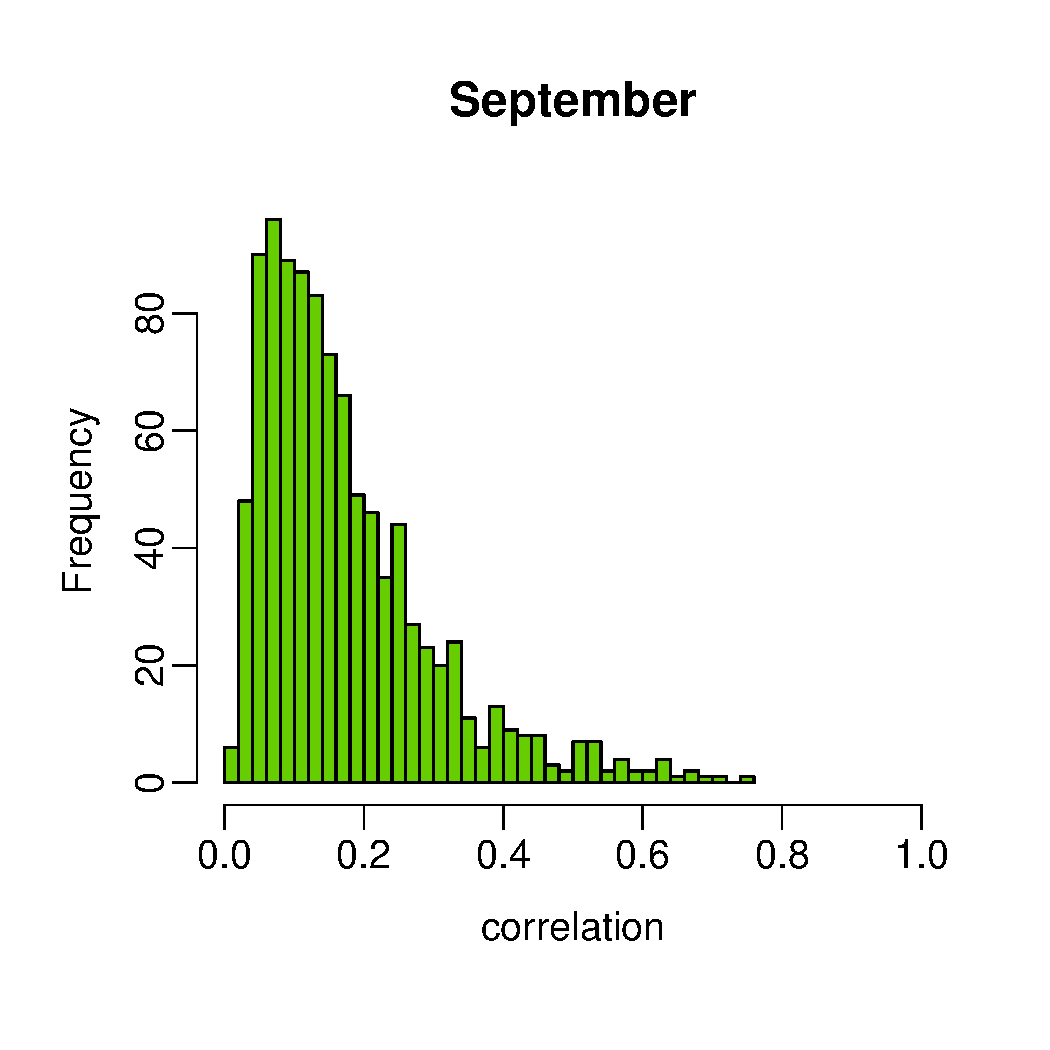
\includegraphics[width=\scale]{Validation_Plots/Correlation/Correlation_09_Sep}\\[-3ex]
 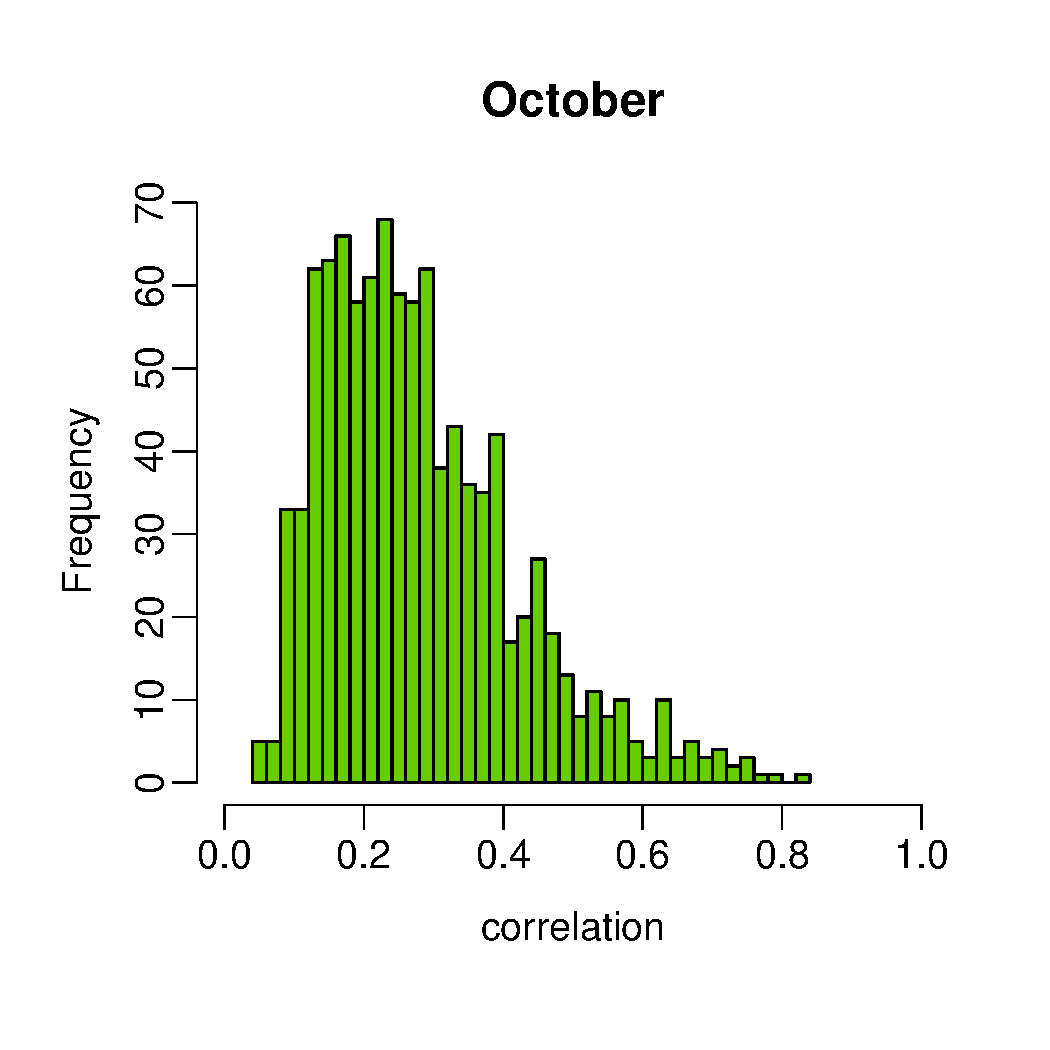
\includegraphics[width=\scale]{Validation_Plots/Correlation/Correlation_10_Oct}\hspace{-1ex}
 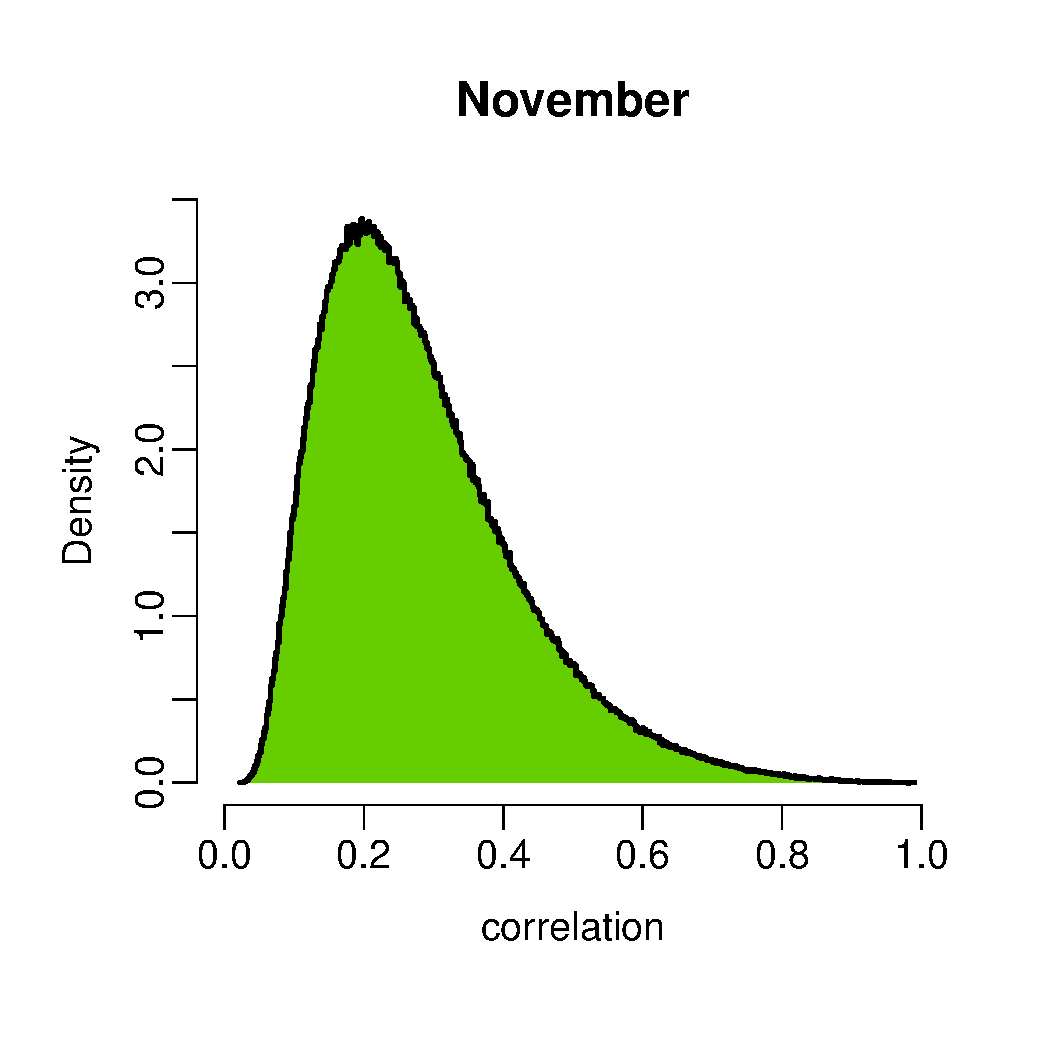
\includegraphics[width=\scale]{Validation_Plots/Correlation/Correlation_11_Nov}\hspace{-1ex}
 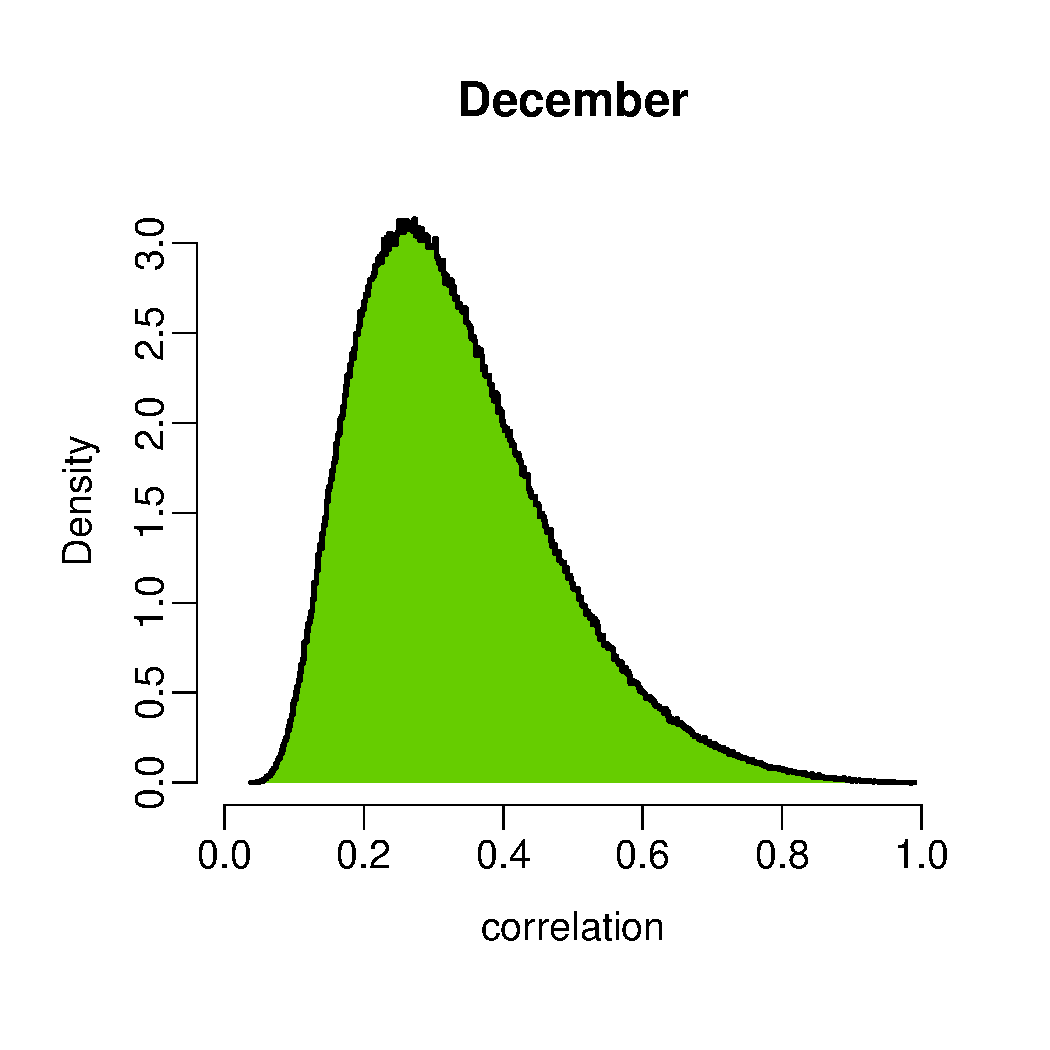
\includegraphics[width=\scale]{Validation_Plots/Correlation/Correlation_12_Dec}
 \caption{Histograms of the correlations between the point at the center of the hypercube $[-1,1]^N$ (where, for each month, $N$ is the number of active inputs) and $2\times 10^6$ uniformly distributed points in the hypercube.}
 \label{Fig_Correlation}
\end{figure}



\section{Emulators' Validation and Exploration}\label{Validation}
This section concerns the validation of the previously built emulators. Choices of the active inputs and hyperparameters have been made based on the performance of the emulators on an evaluation set consisting of 150 observations not used in training. The emulators built this way have then been used to predict the simulated values of a completely new test set, consisting of additional 150 observations. 

\renewcommand{\scale}{12.7em}
\begin{figure}
\centering

 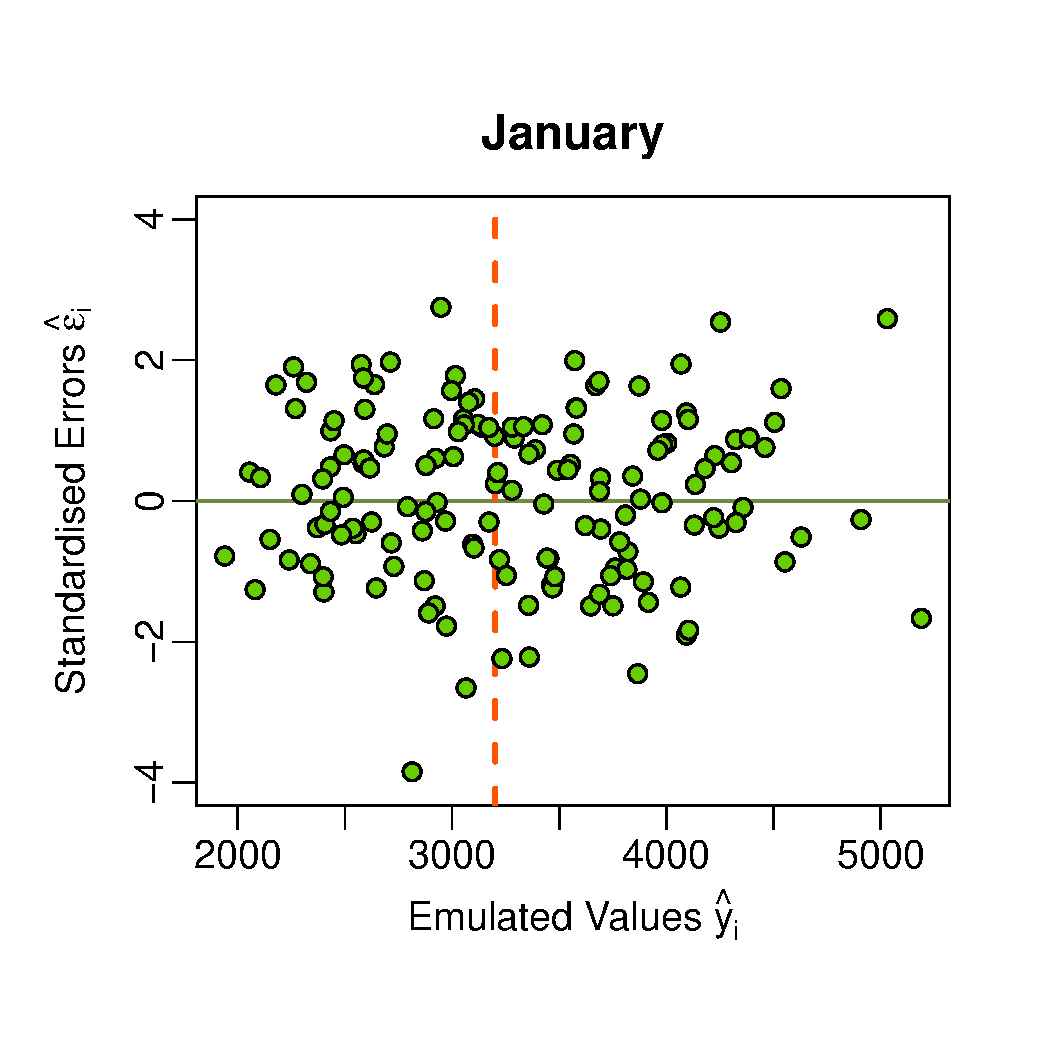
\includegraphics[width=\scale]{Validation_Plots/Evaluation_Set/Evaluation_Scatter_01_Jan}\hspace{-1ex}
 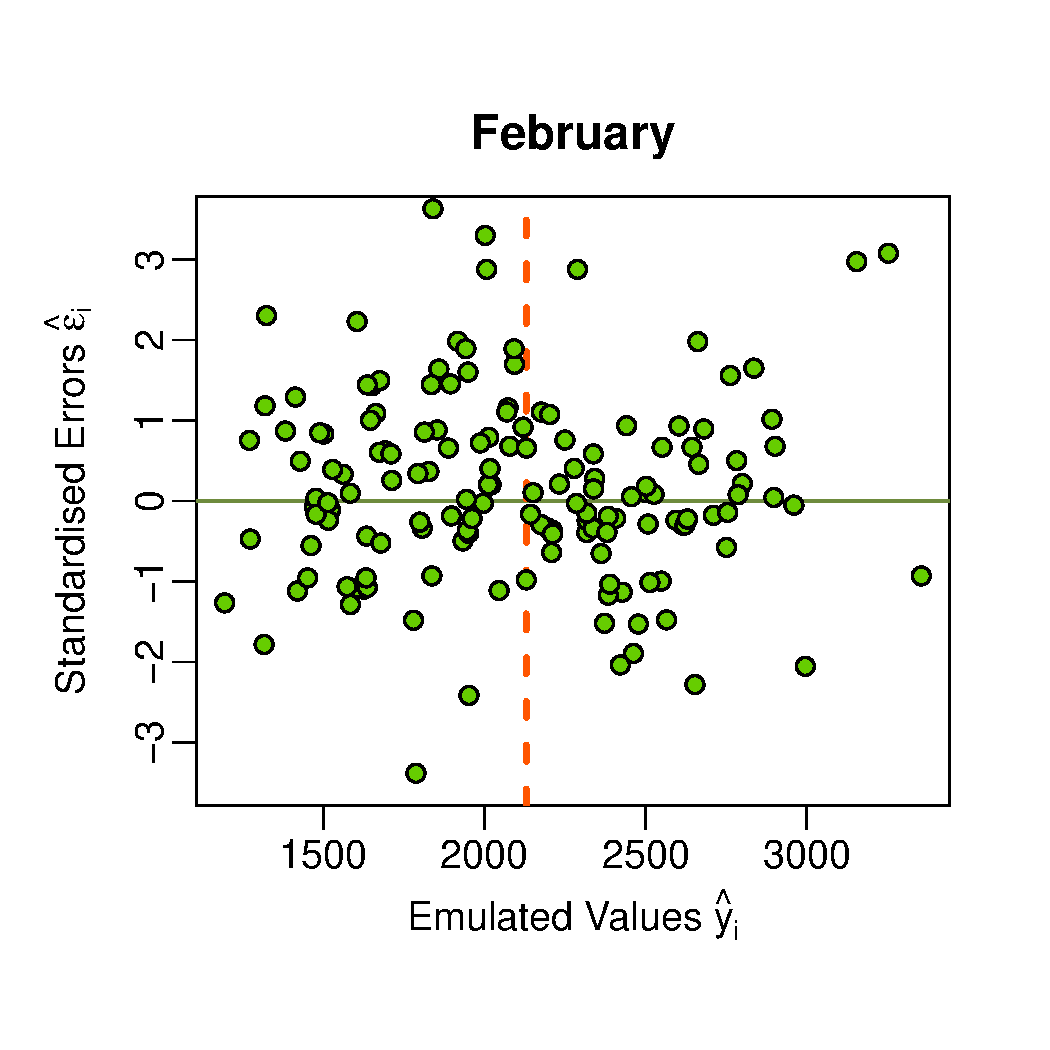
\includegraphics[width=\scale]{Validation_Plots/Evaluation_Set/Evaluation_Scatter_02_Feb}\hspace{-1ex}
 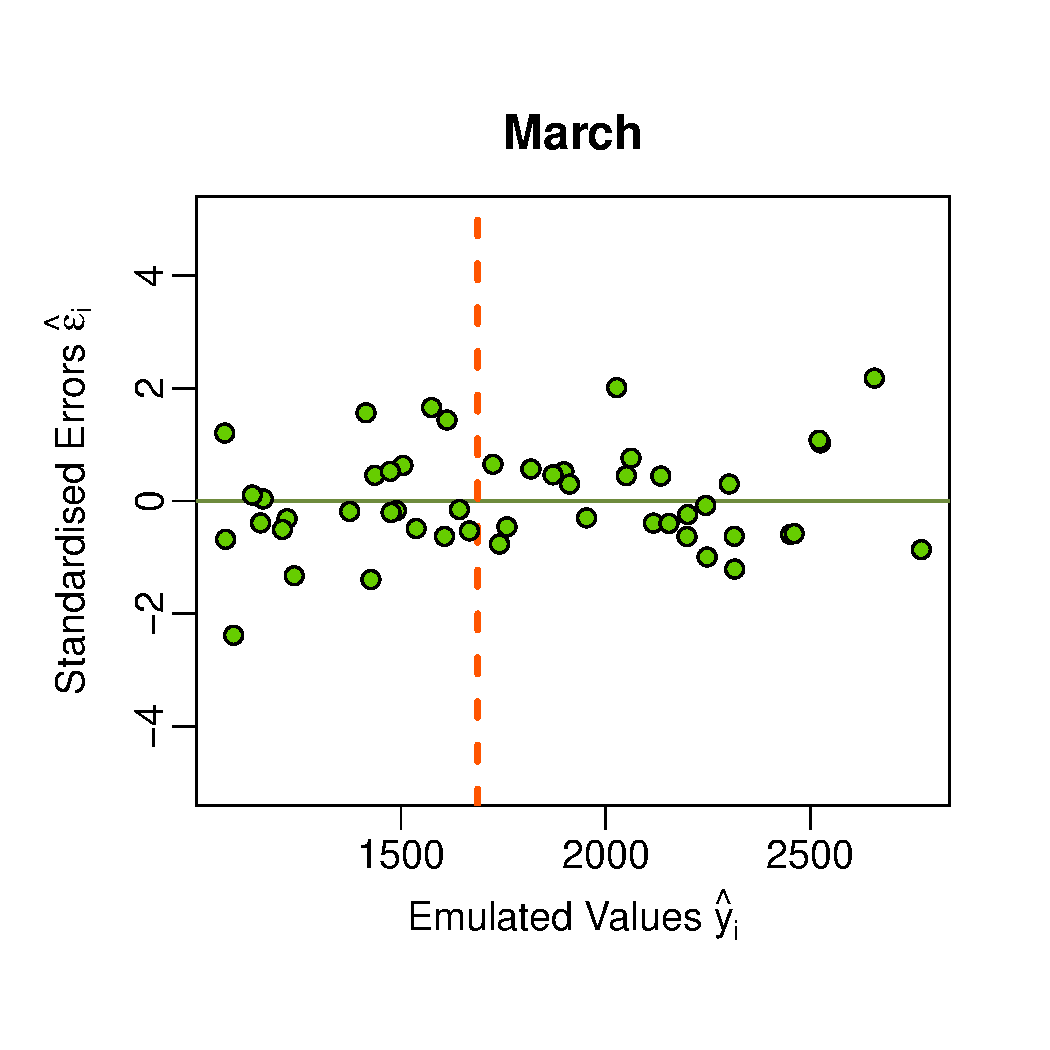
\includegraphics[width=\scale]{Validation_Plots/Evaluation_Set/Evaluation_Scatter_03_Mar}\\[-3ex]
 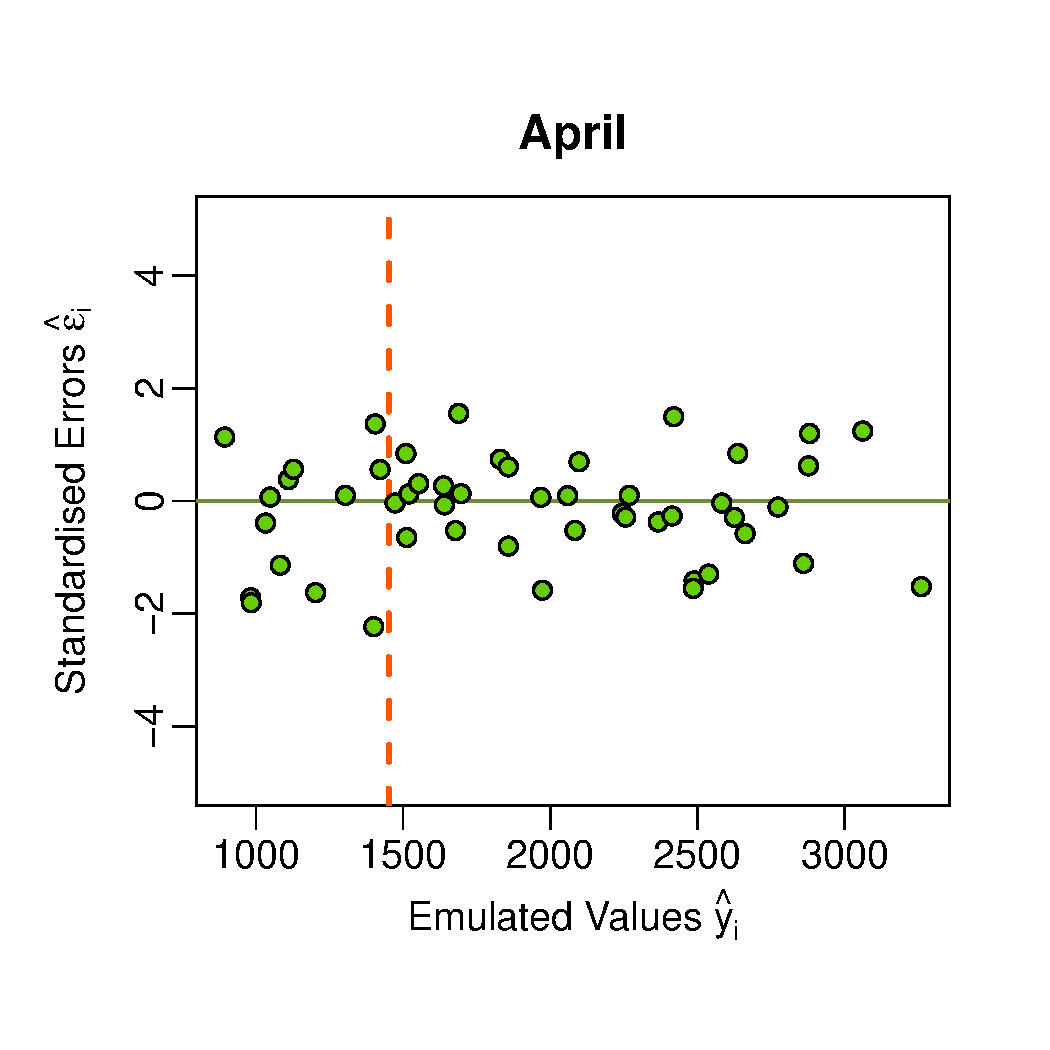
\includegraphics[width=\scale]{Validation_Plots/Evaluation_Set/Evaluation_Scatter_04_Apr}\hspace{-1ex}
 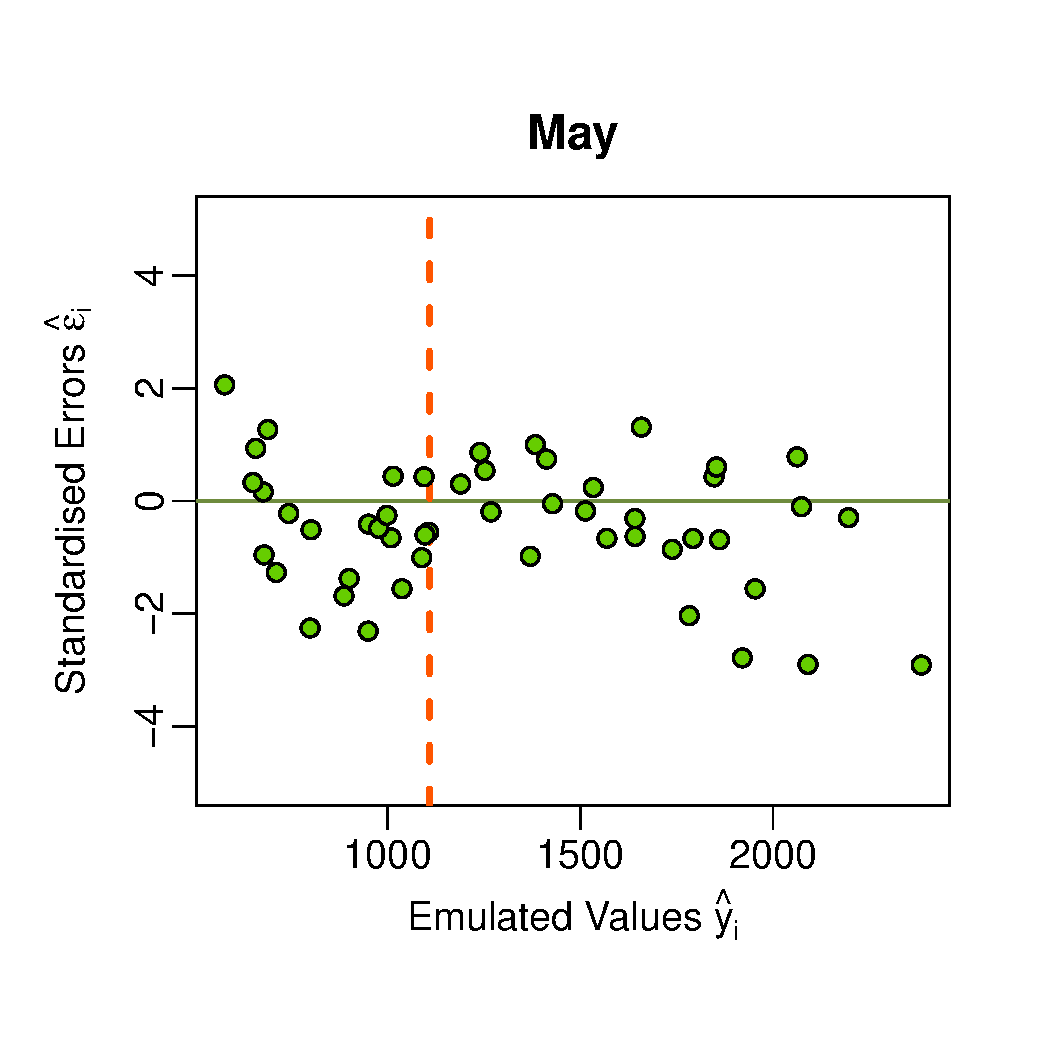
\includegraphics[width=\scale]{Validation_Plots/Evaluation_Set/Evaluation_Scatter_05_May}\hspace{-1ex}
 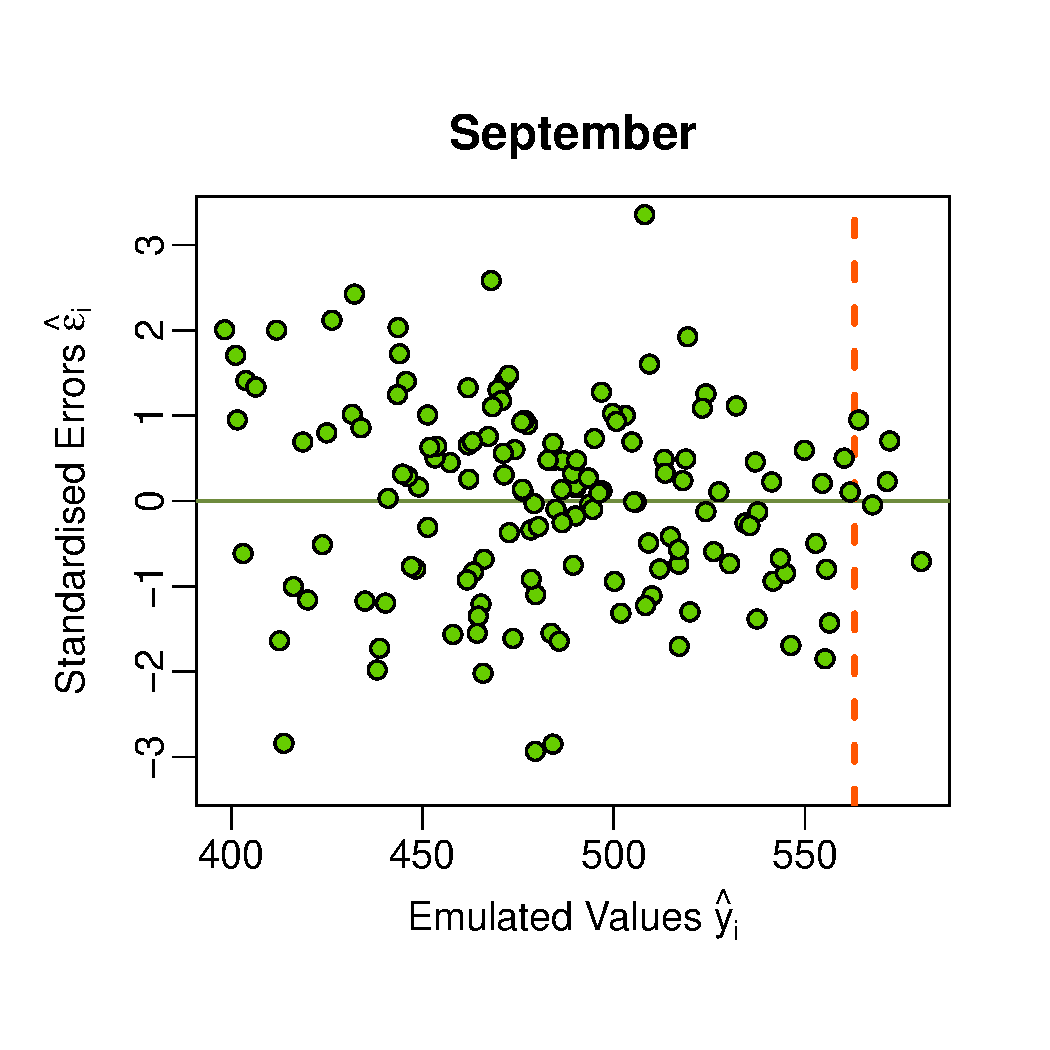
\includegraphics[width=\scale]{Validation_Plots/Evaluation_Set/Evaluation_Scatter_09_Sep}\\[-3ex]
 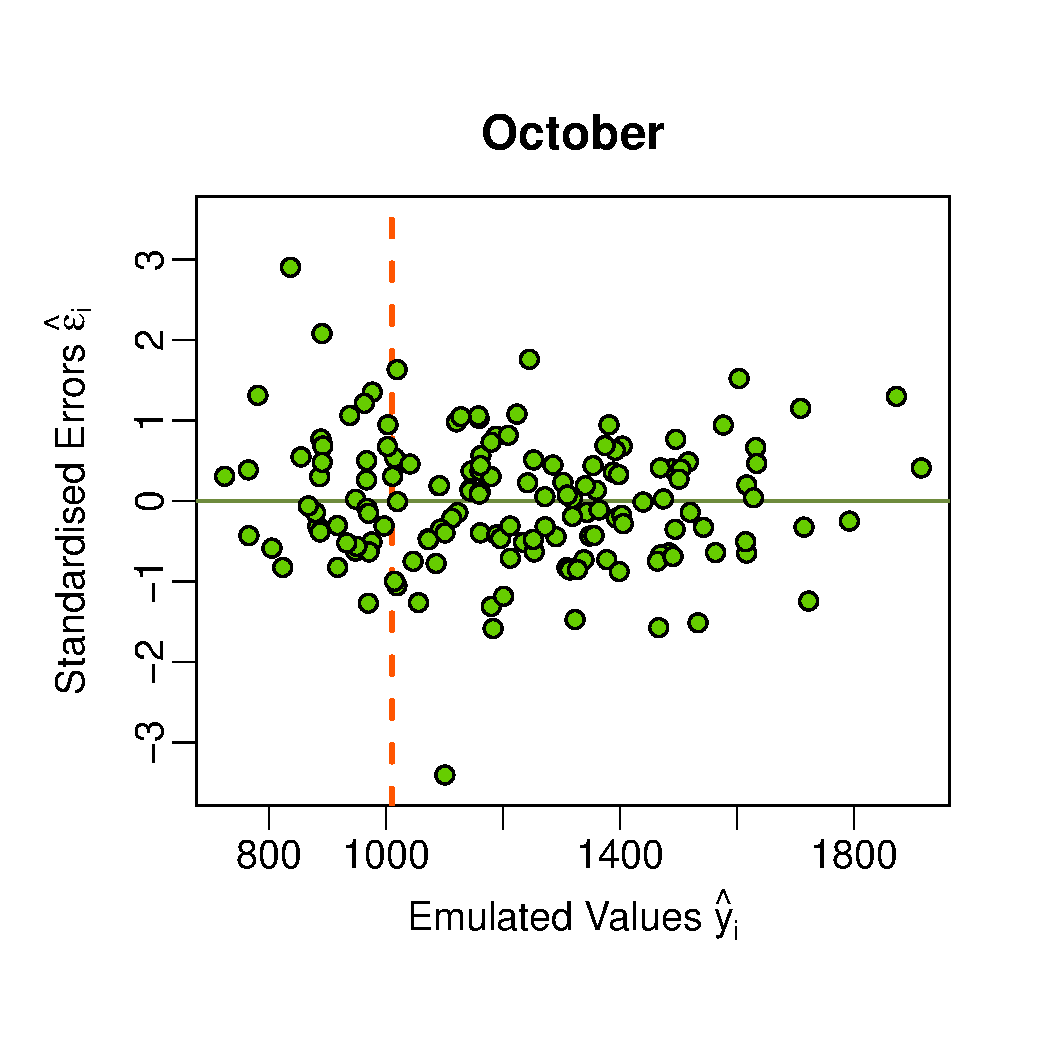
\includegraphics[width=\scale]{Validation_Plots/Evaluation_Set/Evaluation_Scatter_10_Oct}\hspace{-1ex}
 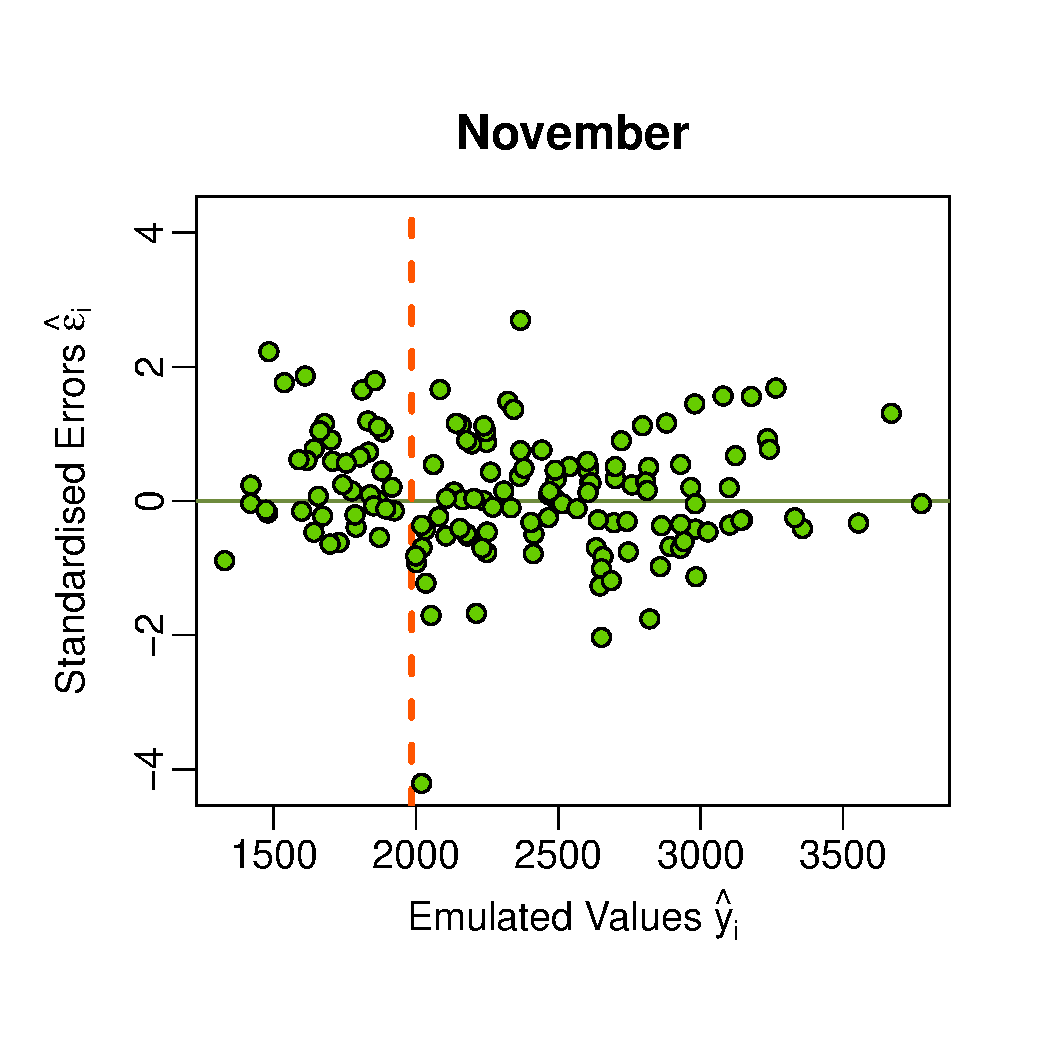
\includegraphics[width=\scale]{Validation_Plots/Evaluation_Set/Evaluation_Scatter_11_Nov}\hspace{-1ex}
 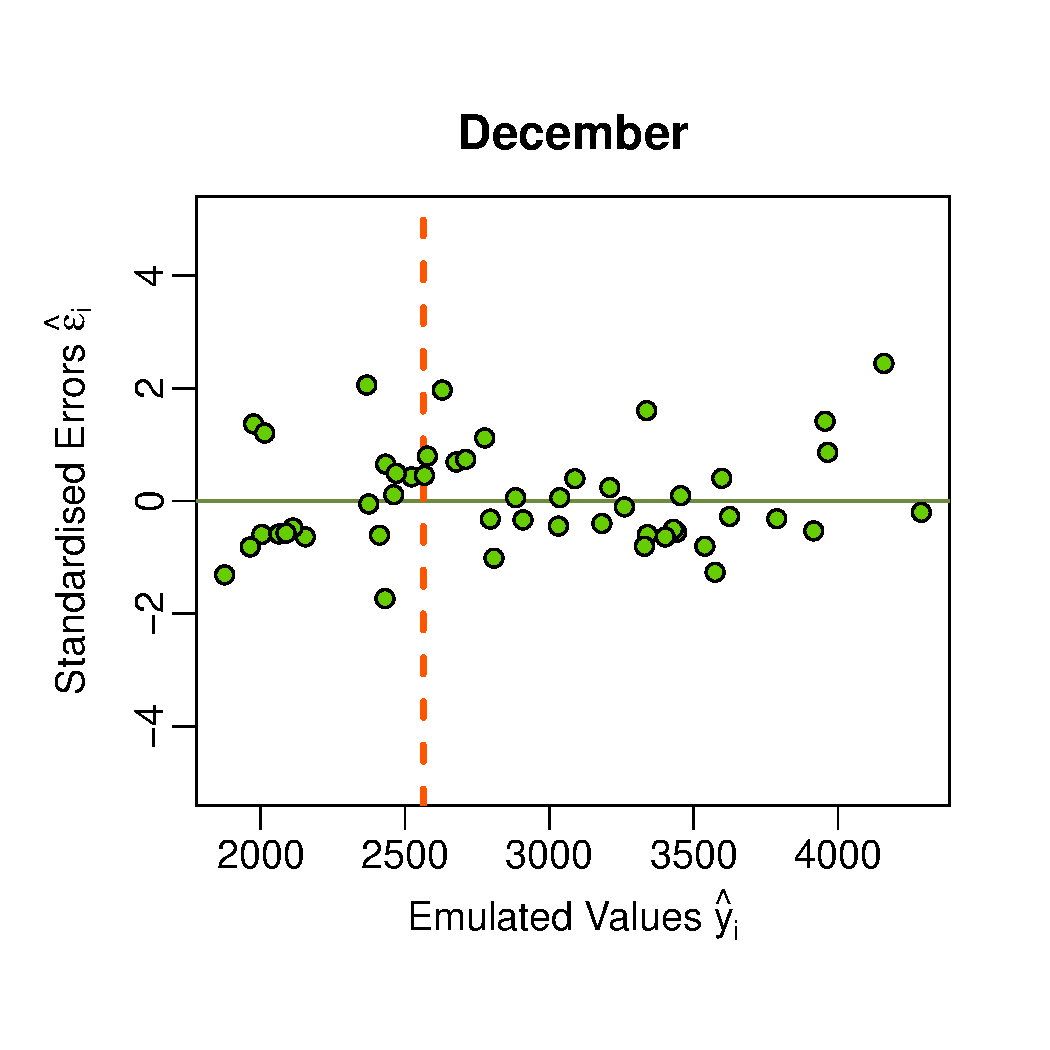
\includegraphics[width=\scale]{Validation_Plots/Evaluation_Set/Evaluation_Scatter_12_Dec}
 \caption{Validation of the emulators on the evaluation set, consisting of 150 points not used in training. For the different months, the standardised errors in \eqref{Eqn_St_Er} are plotted against the emulator's fitted values. In each plot, the vertical dashed line identifies the value on the $x$-axis corresponding to the observed gas consumption for the month.}
 \label{Fig_Scatter_Errors_Eval}
\end{figure}


\autoref{Fig_Scatter_Errors_Eval} and \autoref{Fig_Scatter_Errors_Test} show the emulated standardised errors on the evaluation and test sets respectively. For any point in such sets, call $y_i$ the known simulator response, $\hat{y}_i$ the emulator prediction and $\hat{\sigma}_i$ the associated standard deviation. The standardised error is computed as follows:
\begin{equation}\label{Eqn_St_Er}
\hat{\eps}_i = \frac{y_i - \hat{y}_i}{\hat \sigma_i}.
\end{equation}

Values of the emulator hyperparameters have been chosen so that the standardised errors in \autoref{Fig_Scatter_Errors_Eval} would display as unstructured as possible patterns, and at least 95\% of them would be lower than 3 in modulus. We consider the plots in \autoref{Fig_Scatter_Errors_Eval} satisfactory in this regard. Only the plot concerning May displays a few larger errors, particularly for low $\hat y$ values. This may be a sign that the simulator response varies non-linearly between parts of the space corresponding to smaller and bigger $y$ values. Moreover, further investigation shows that the point with lowest (negative) $\hat \eps$ in the seven plots January--April and October-December corresponds to the same choice of inputs in all cases. The point, then, may be considered an outlier with respect to the emulator models, although its standardised errors rarely go beyond the value $-4$. As to all other points, their standardised errors are essentially comprised between $-3$ and $+3$. 

The plots in \autoref{Fig_Scatter_Errors_Test} show the standardised errors of a set of completely new points, not used in training or evaluation. The plots show that the magnitude and pattern of the standardised errors are satisfactory for the test set too, so we consider the emulators successfully validated.


\begin{figure}
\centering
 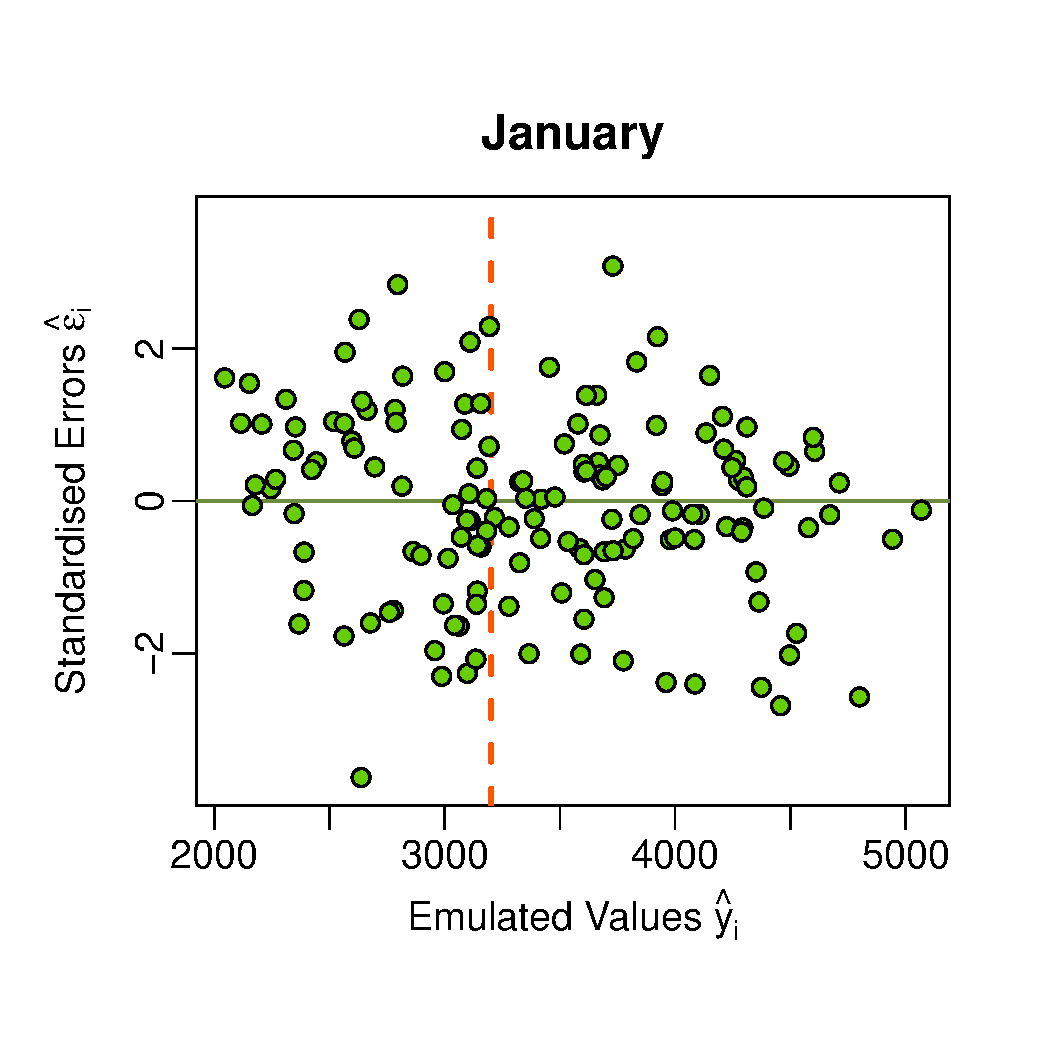
\includegraphics[width=\scale]{Validation_Plots/Test_Set/Test_Scatter_01_Jan}\hspace{-1ex}
 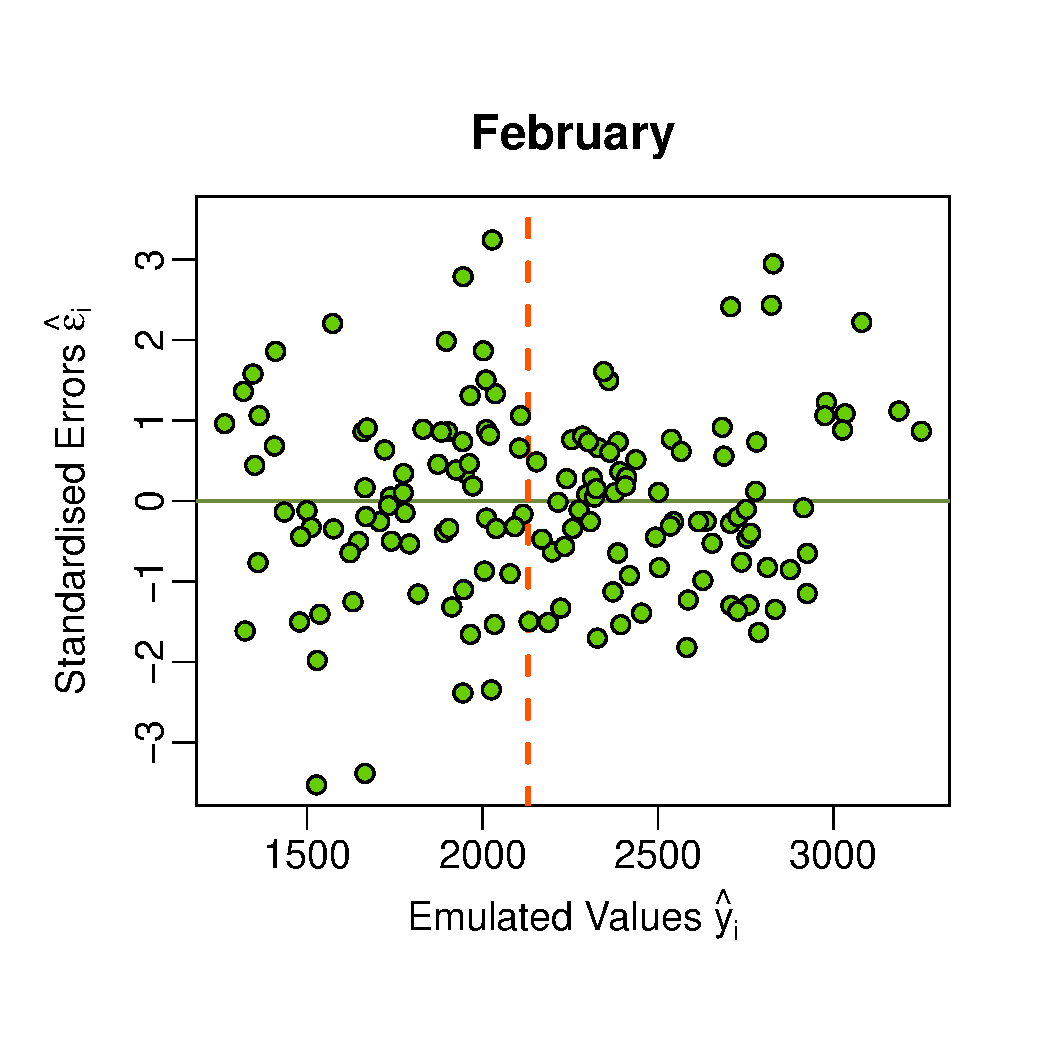
\includegraphics[width=\scale]{Validation_Plots/Test_Set/Test_Scatter_02_Feb}\hspace{-1ex}
 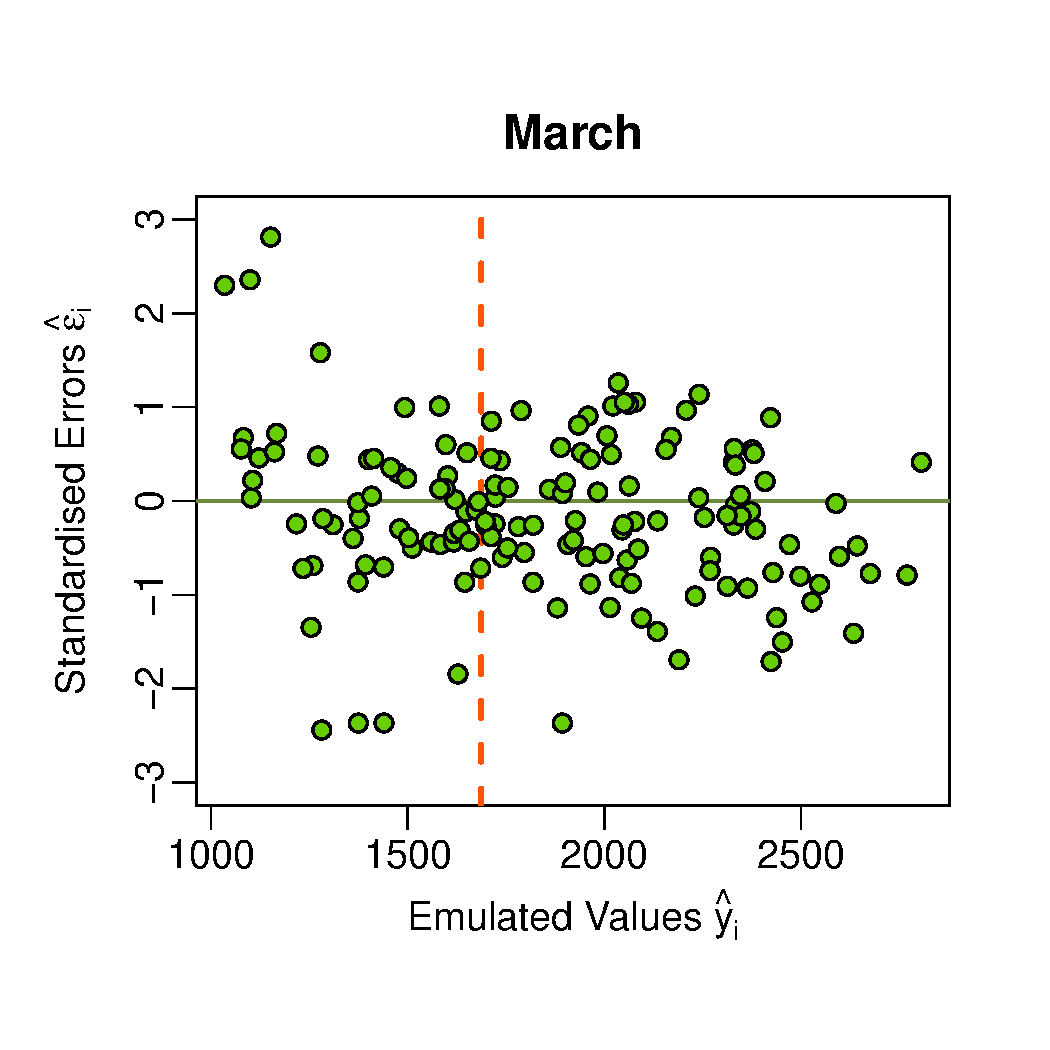
\includegraphics[width=\scale]{Validation_Plots/Test_Set/Test_Scatter_03_Mar}\\[-3ex]
 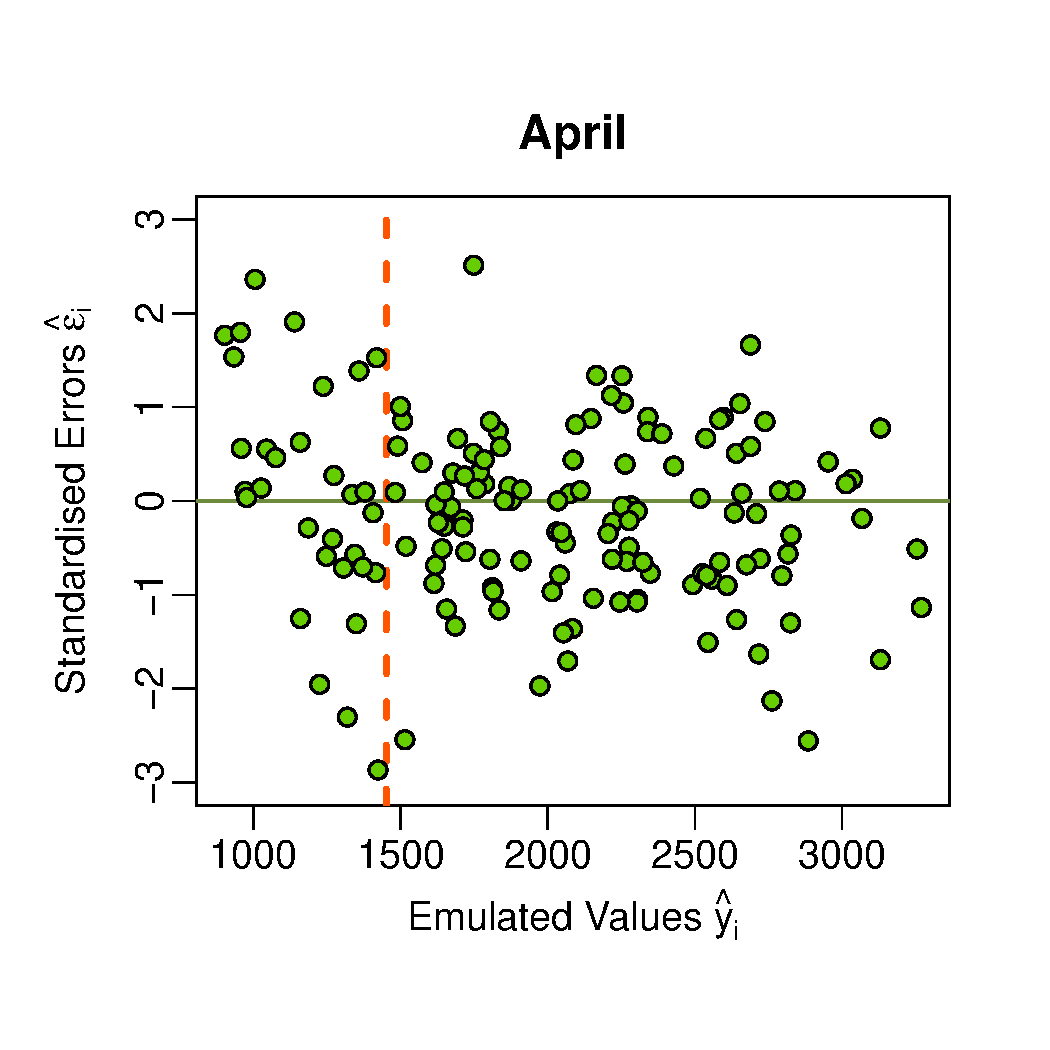
\includegraphics[width=\scale]{Validation_Plots/Test_Set/Test_Scatter_04_Apr}\hspace{-1ex}
 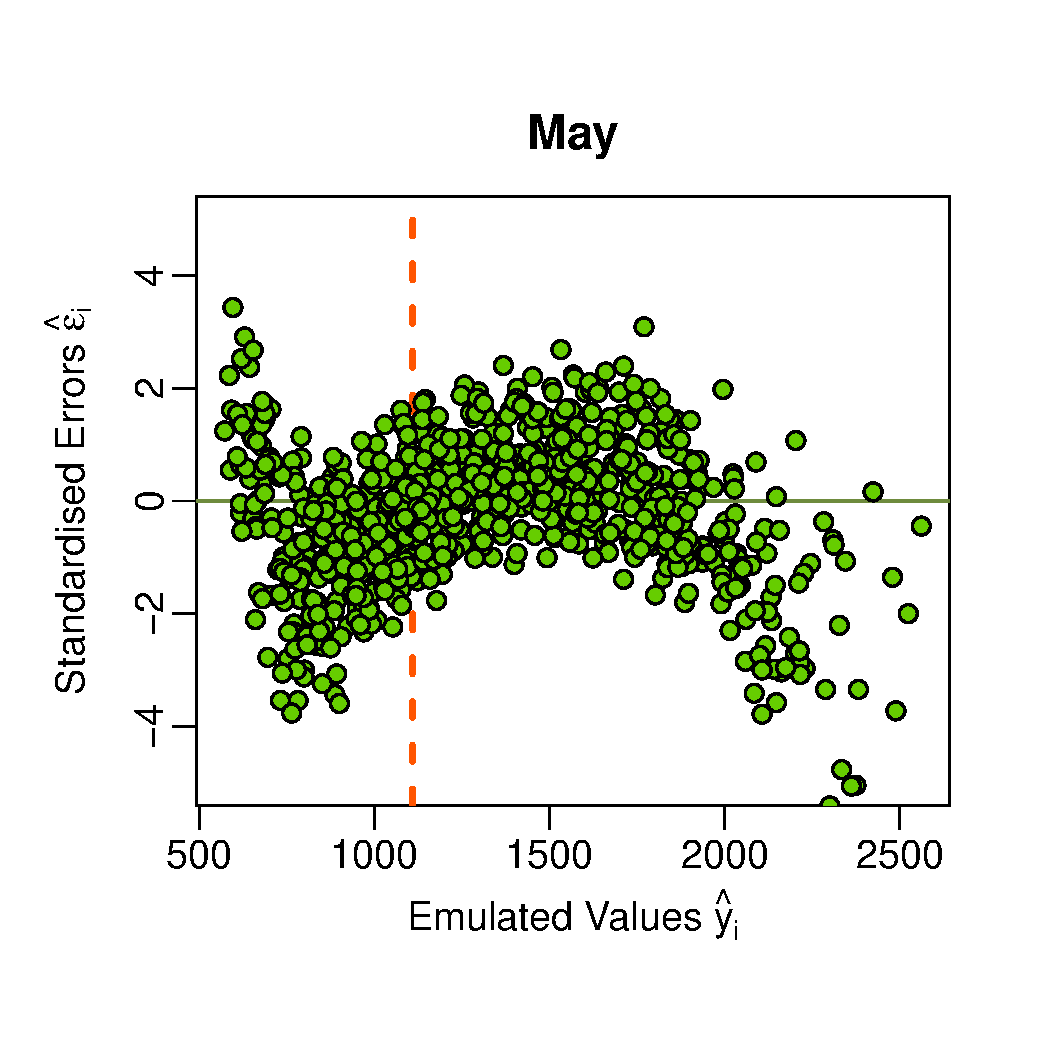
\includegraphics[width=\scale]{Validation_Plots/Test_Set/Test_Scatter_05_May}\hspace{-1ex}
 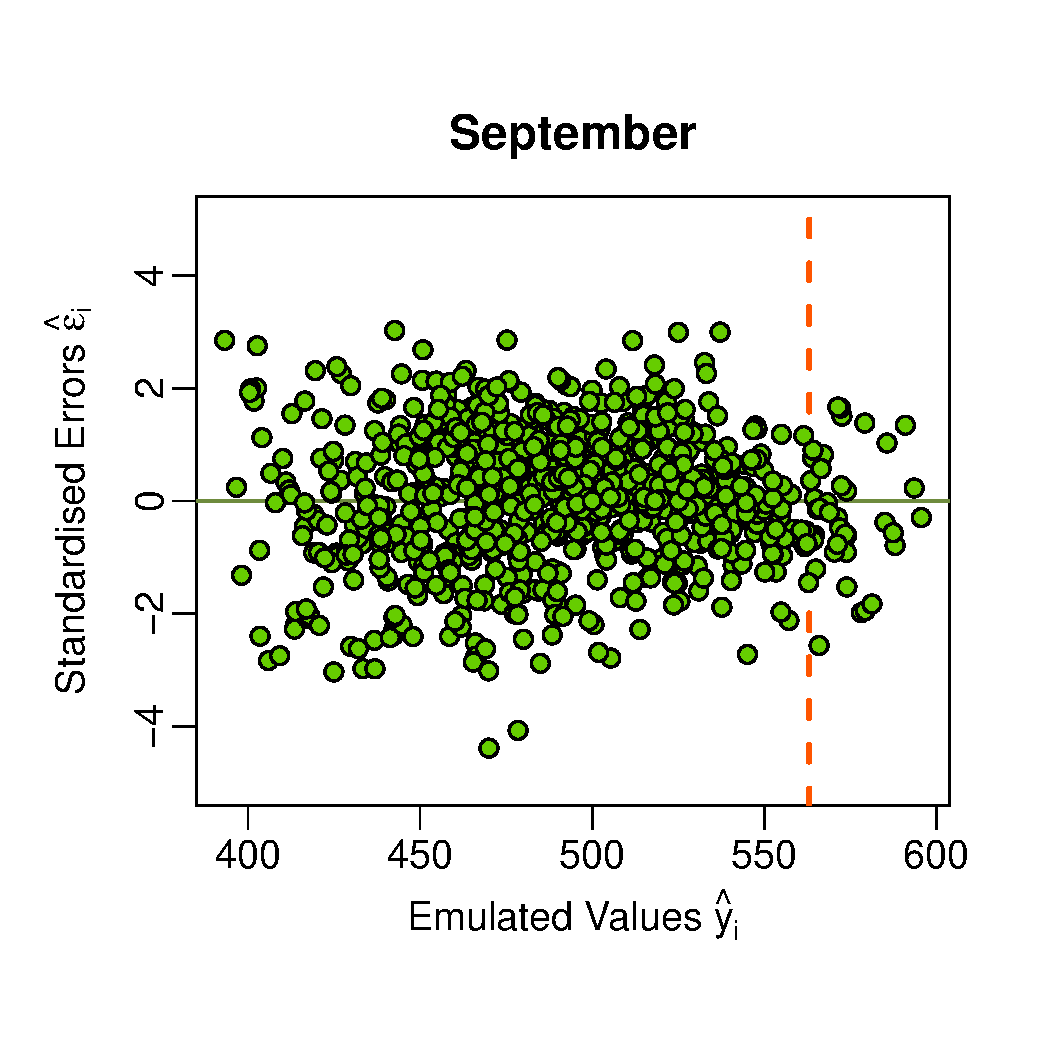
\includegraphics[width=\scale]{Validation_Plots/Test_Set/Test_Scatter_09_Sep}\\[-3ex]
 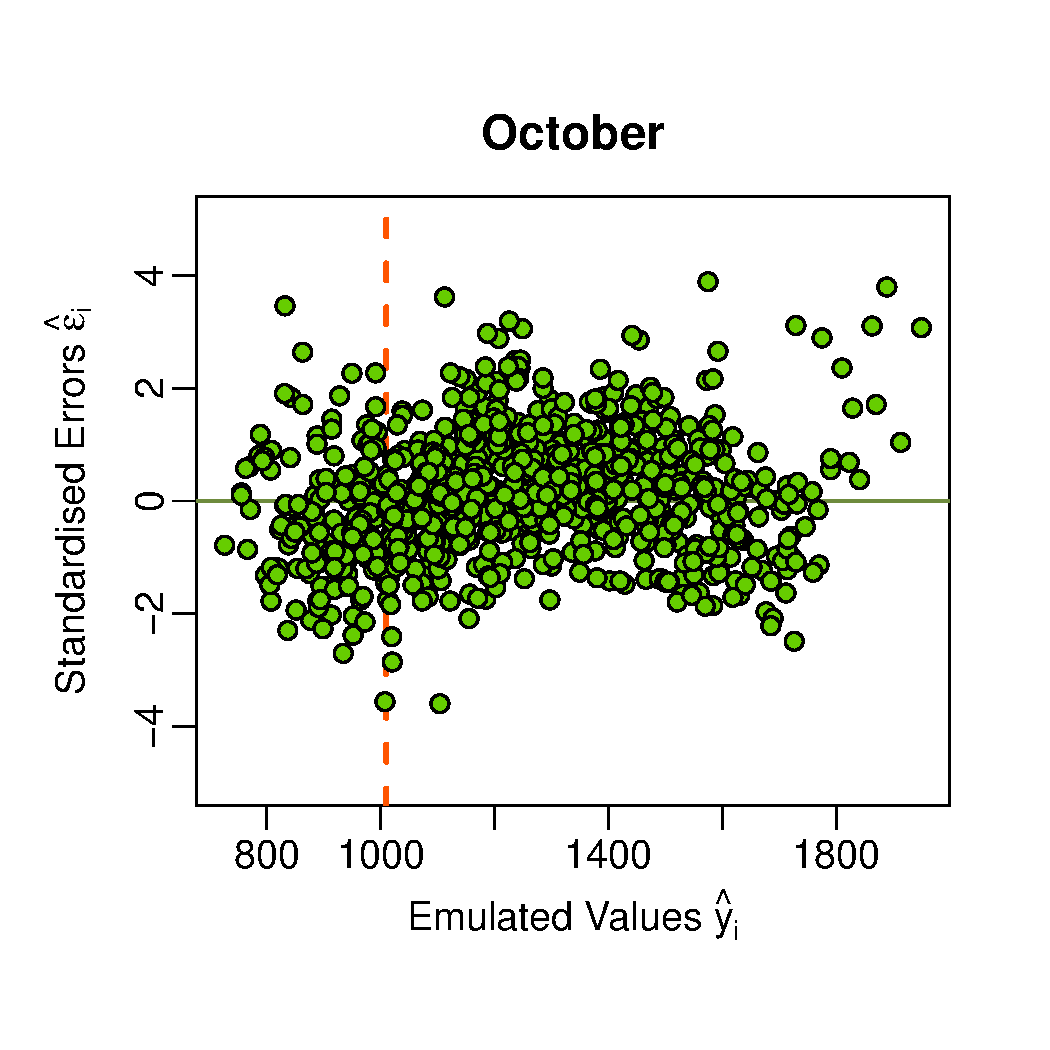
\includegraphics[width=\scale]{Validation_Plots/Test_Set/Test_Scatter_10_Oct}\hspace{-1ex}
 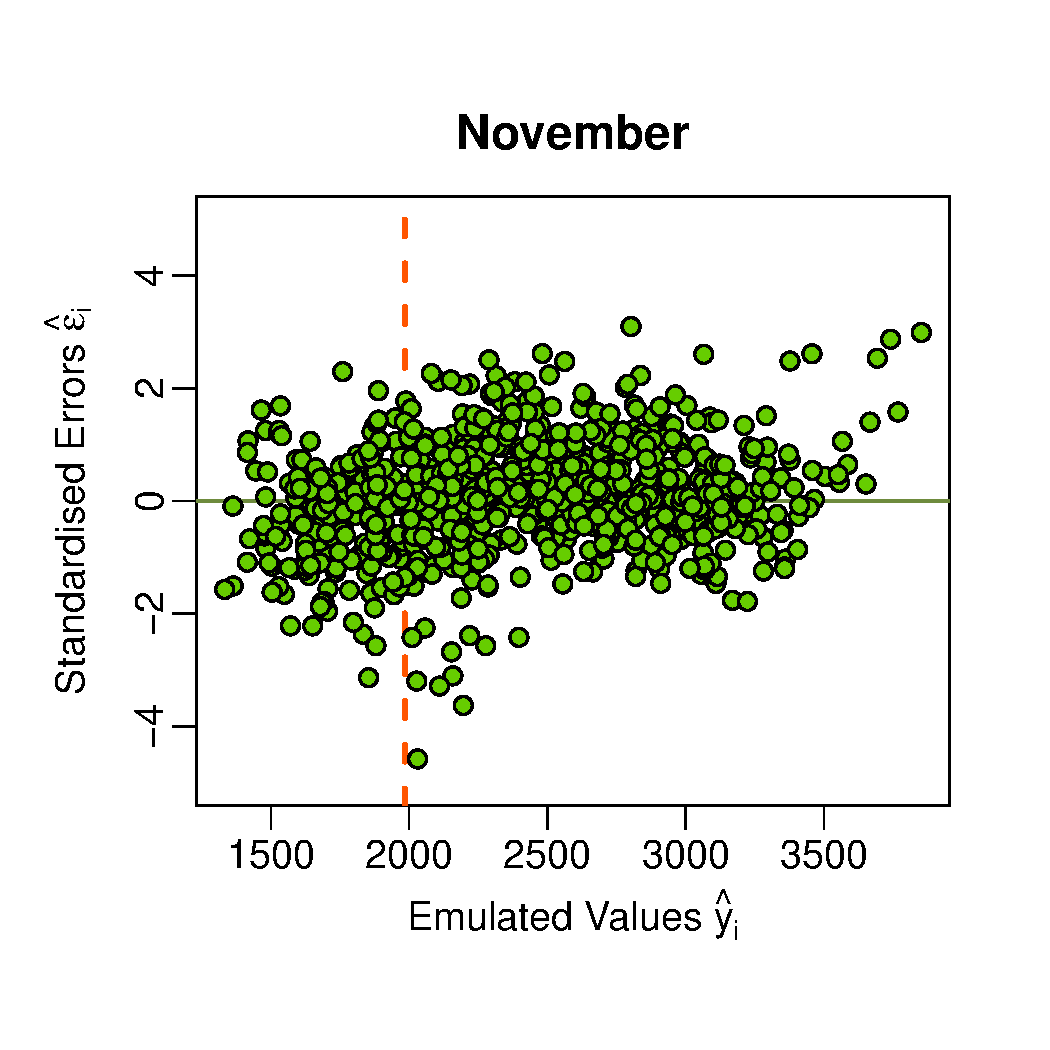
\includegraphics[width=\scale]{Validation_Plots/Test_Set/Test_Scatter_11_Nov}\hspace{-1ex}
 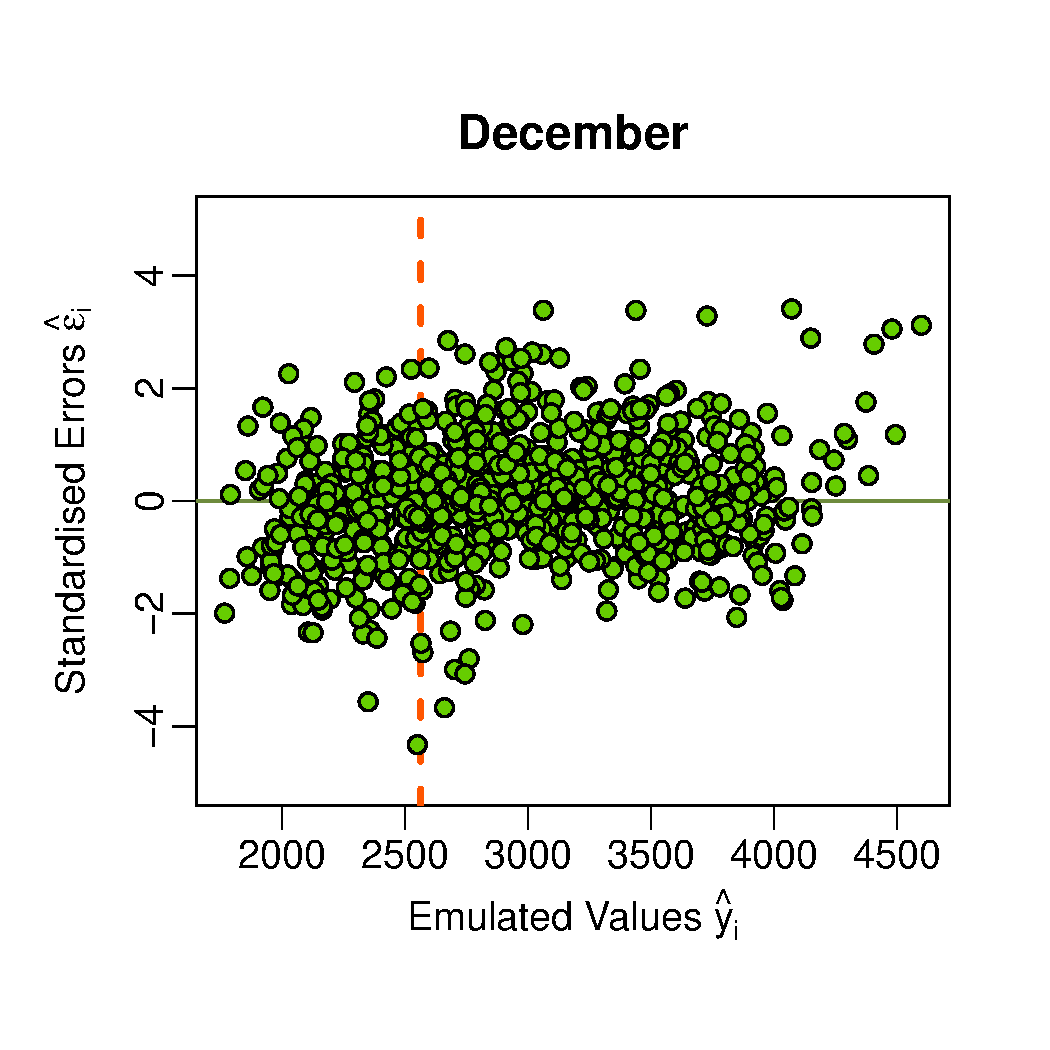
\includegraphics[width=\scale]{Validation_Plots/Test_Set/Test_Scatter_12_Dec}
\caption{Validation of the emulators on the test set, consisting of 150 points not used in training and evaluation. For the different months, the standardised errors in \eqref{Eqn_St_Er} are plotted against the emulator's fitted values. In each plot, the vertical dashed line identifies the value on the $x$-axis corresponding to the observed gas consumption for the month.}
 \label{Fig_Scatter_Errors_Test}
\end{figure}


\subsection{Comparison Between LR and Trained Emulators}

For each month, \autoref{Table_sigma} compares the prior variance of the emulator (\ie, the variance of the original linear regression residuals) with the adjusted variance of the emulator predictions on the 150 test points. I am reporting the $2.5$ and $97.5$ empirical percentiles of these, to get a sense of the difference in prediction uncertainty between the original linear regression and the trained emulators.

\begin{table}
 \centering
 \renewcommand{\arraystretch}{1.7}
 \newcommand{\colsep}{3ex}
 \tabcolsep=6pt
 \caption{For each month: the first line of the table shows the variance of the linear regression residuals (prior cumulative variance of the emulator). The second and third lines show the $2.5$ and $97.5$ empirical percentiles of the emulator variances at the 150 test points.}
 \begin{tabular}{c<{\hspace{\colsep}}ccccccccc}
\specialrule{.1em}{0em}{0.1em} 
 &  \textbf{Jan} & \textbf{Feb} & \textbf{Mar} & \textbf{Apr} & \textbf{May} & \textbf{Sep} & \textbf{Oct} & \textbf{Nov} & \textbf{Dec}\\
 \specialrule{.05em}{.1em}{0.1em} 
 \specialrule{.05em}{0em}{0.2em} 
  $\sigma^2$  & 85.9 &  52.3  &  50.1 &  50.0  & 206.4  &  0.91 &  24.4  & 57.4  &  68.8\\
  $[2.5\%$,       & 6.6   & 5.9     &  3.1   & 3.2      & 16.8    & 0.06  & 1.46   & 3.8    & 4.3\\
  $97.5\%]$ CI & 31.0 & 28.0   & 9.3    & 10.0   & 68.9    &  0.20 & 3.80   & 12.8  & 12.7\\
 \specialrule{.1em}{0.2em}{1em} 
 \end{tabular}
\label{Table_sigma}
\end{table}

Finally, \autoref{Fig_Comparison_LR} allows to compare graphically the accuracy of the emulator's predictions versus the linear regression's ones. The plot concerns the month of March. Results for only 8 of the 150 test points are shown (8 consecutive ones in terms of the simulator outputs), to avoid cluttering which would prevent details to be appreciated. 

The red ``cat's eye'' boxes represent the emulator predictions for these points, within a range of three standard deviations from the mean prediction. The blue plus sign and the yellow squares represent instead the real simulator outputs and the linear regression predictions, respectively. It can be appreciated that the emulator is often much more precise than the linear model, and has a high level of confidence in its prediction (small uncertainty bands).




\begin{figure}
\centering
 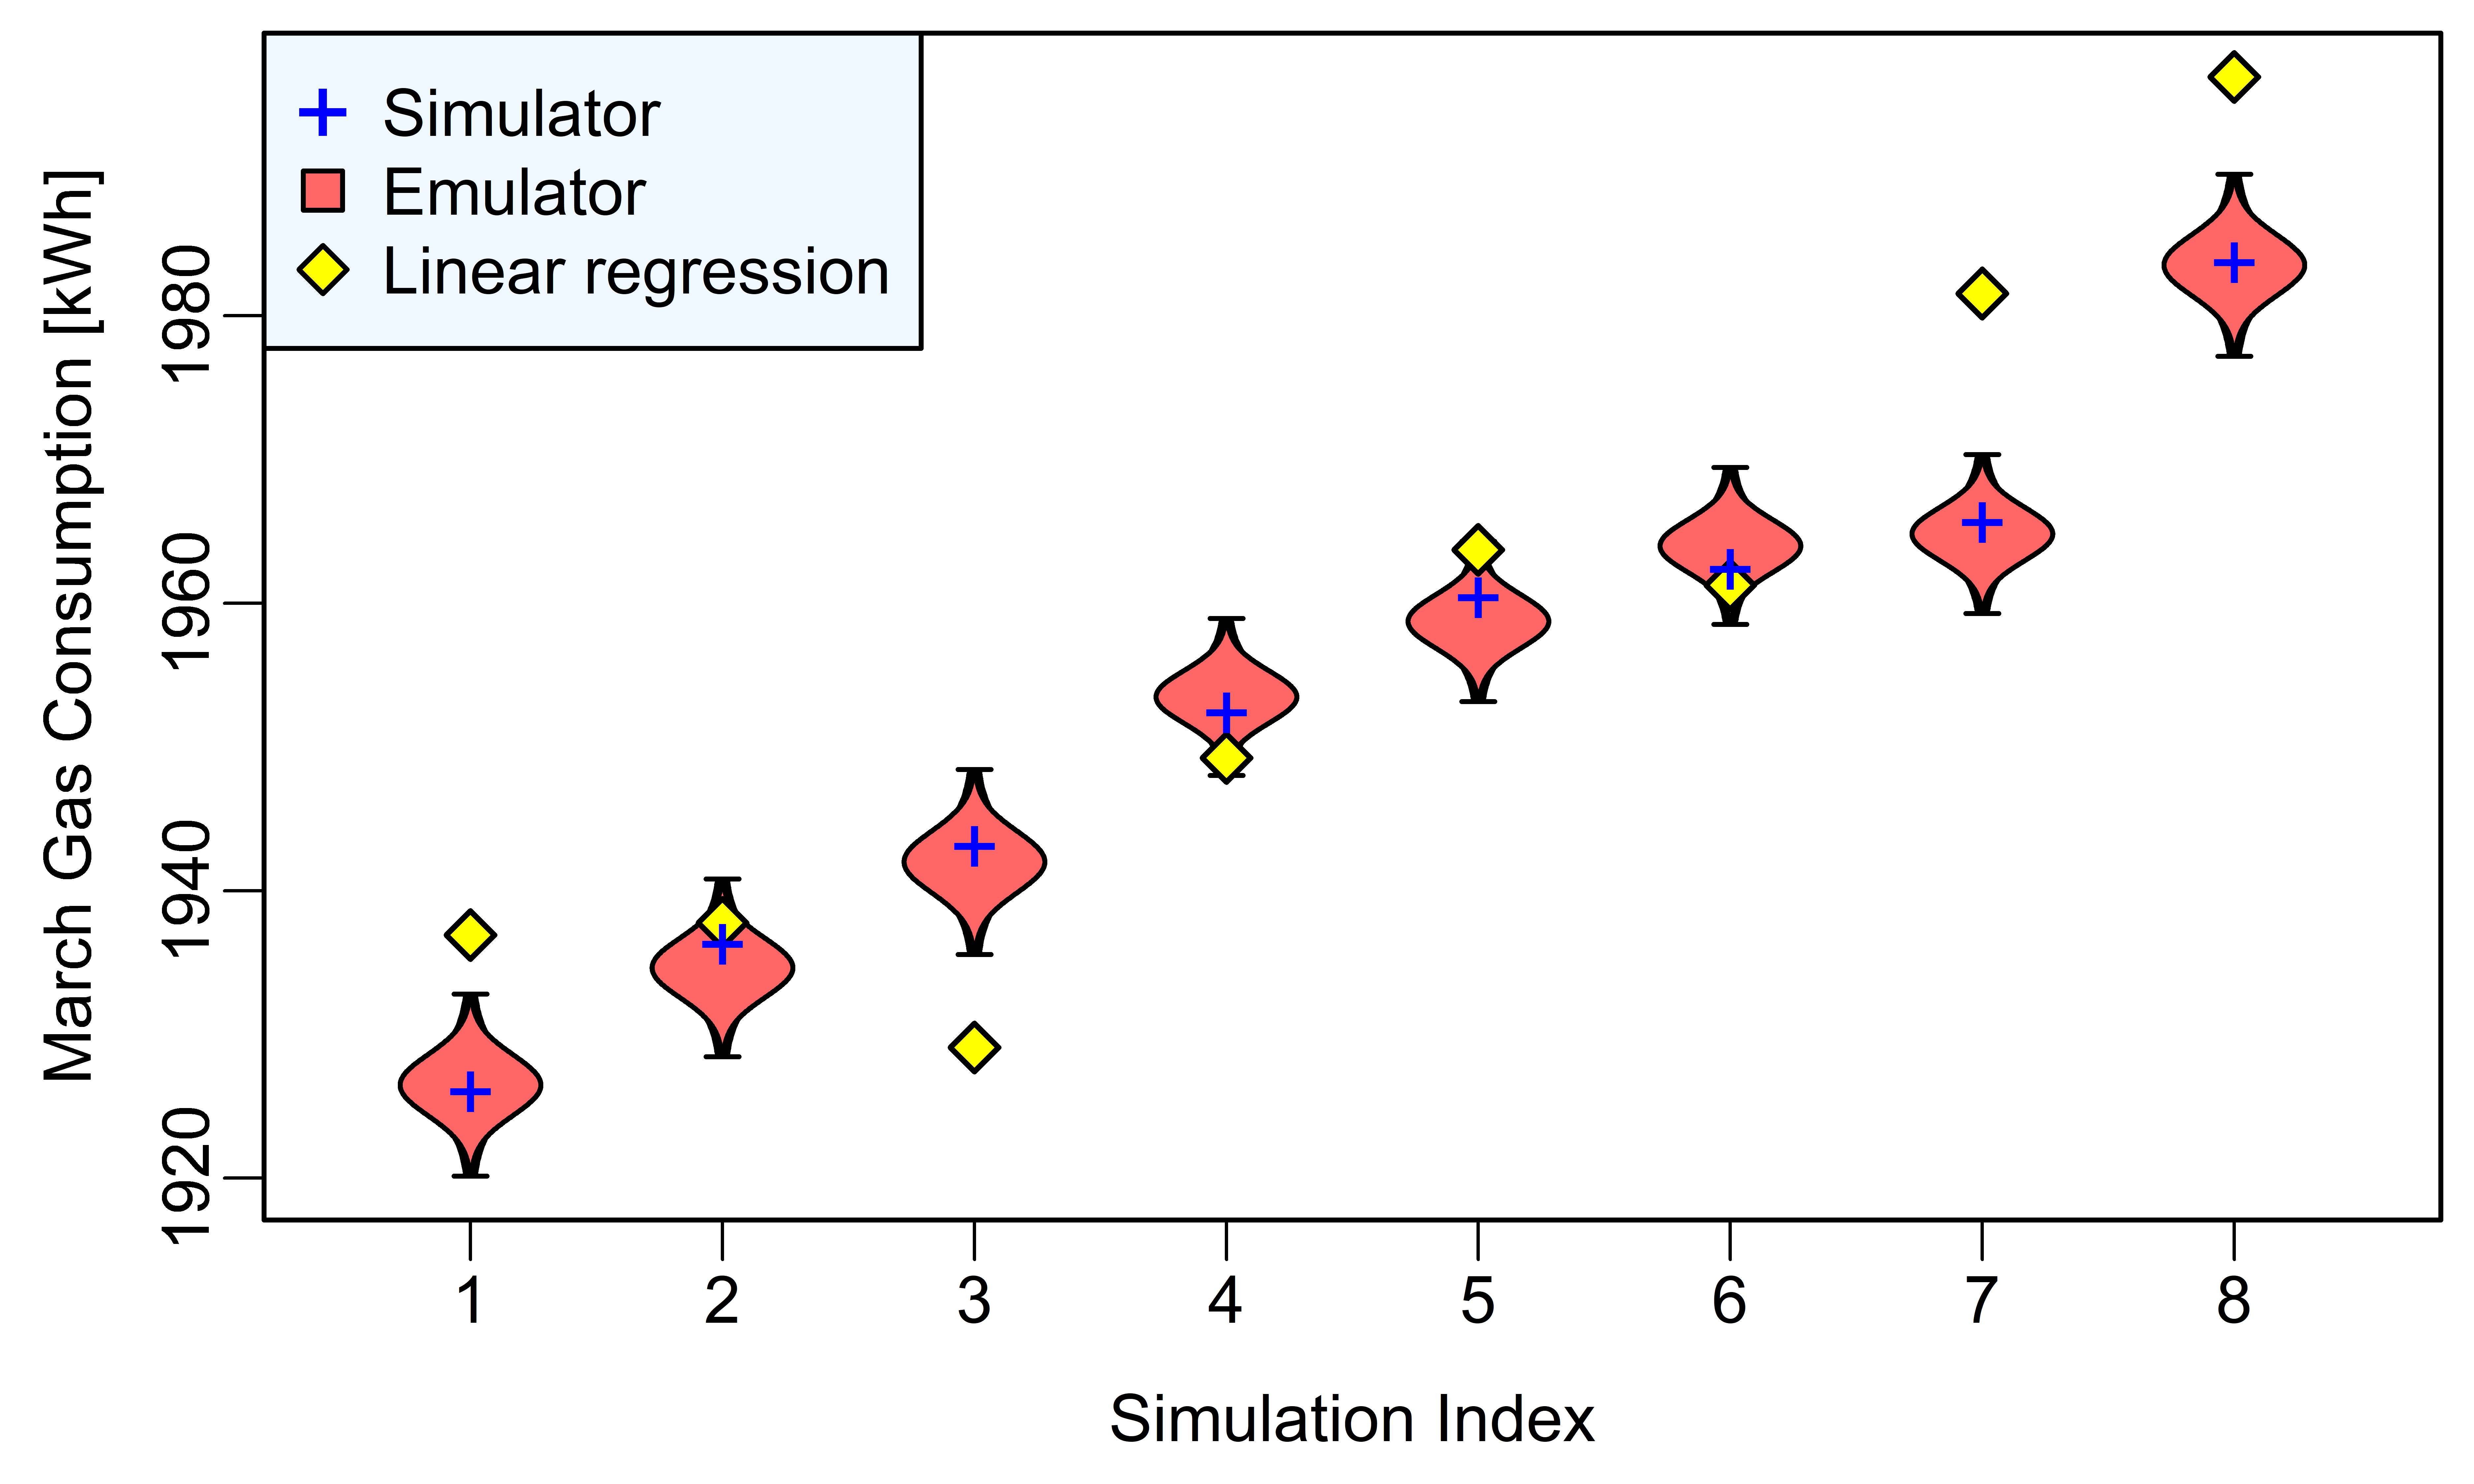
\includegraphics[width=0.8\textwidth]{Validation_Plots/Comparison_LR/LR_Mar_82-89}
 \caption{Visual comparison between emulator (red cat's eye boxes) and linear regression (yellow squares) predictions. The plot concerns 8 points of the test set for the month of March. The height of the emulator cat's eye boxes covers a range of three standard deviations from the emulator's mean prediction. This range always includes the simulated value (blue plus sign), and often represents a much more precise prediction than the original linear regression one.}
 \label{Fig_Comparison_LR}
\end{figure}







\end{document}
